\documentclass[phd,tocprelim]{cornell}
%% Added to avoid the \ifpdf name clash error
\let\ifpdf\relax
%
% tocprelim option must be included to put the roman numeral pages in the
% table of contents
%
% The cornellheadings option will make headings completely consistent with
% guidelines.
%
% This sample document was originally provided by Blake Jacquot, and
% fixed up by Andrew Myers.
%
%Some possible packages to include
\usepackage{graphicx,pstricks}
\usepackage{graphics}
\usepackage{moreverb}
\usepackage{subfigure}
\usepackage{epsfig}
\usepackage{subfigure}
\usepackage{hangcaption}
\usepackage{txfonts}
\usepackage{palatino}
\usepackage{amssymb}
\usepackage{physics}
\usepackage{appendix}
\usepackage[...]{microtype}
\usepackage[all]{nowidow}
%if you're having problems with overfull boxes, you may need to increase
%the tolerance to 9999
\tolerance=9999
\widowpenalty10000

\bibliographystyle{plain}
%\bibliographystyle{IEEEbib}

\renewcommand{\caption}[1]{\singlespacing\hangcaption{#1}\normalspacing}
\renewcommand{\topfraction}{0.85}
\renewcommand{\textfraction}{0.1}
\renewcommand{\floatpagefraction}{0.75}

\title {Scalable Molecular Design Using Reversible Jump MCMC and Stochastic Approximation}
\author {Patrick B. Grinaway}
\conferraldate {May}{2019}
\degreefield {Ph.D.}
\copyrightholder{Patrick B. Grinaway}
\copyrightyear{2019}

\begin{document}

\maketitle
\makecopyright

\begin{abstract}
Despite the existence of useful models for atomic-scale interactions, designing novel molecules (such as drugs) using this information has been extremely difficult. The difficulty results from the nature of the model, which is both extremely high dimensional and multimodal, as well as the nature of the objective function, which is an expectation under this model. In prior work, these models would be leveraged by computing individual expectation values and using these to rank the various molecules. Here, we introduce a joint probability distribution of configurations and chemical states, allowing the simulation to visit different molecular identities as well as different configurations. This introduces the requirement for reversible jump MCMC, as a change in molecular identity results in a change in dimensionality of the configurations. We then combine this approach with the Self-Adjusted Mixture Sampling (SAMS) technique developed by Tan to achieve sampling of chemical identities according to an arbitrary prespecified distribution. We then sought to use the relative free energies of each state as the target distribution, effectively prioritizing favorable chemical states. However, this requires the estimation of free energies. To resolve this, we simultaneously run another MCMC chain that provides online estimates of the necessary free energies. We additionally generate a transdimensional version of nonequilibrium switching amenable to highly parallel hardware setups.
\end{abstract}

\begin{biosketch}
Patrick Grinaway graduated from Lafayette College in 2011 with a Bachelor of Arts in Engineering Studies, focusing on coursework in Electrical and Computer Engineering. While he was attending Lafayette, he became fascinated with modeling complex systems and understanding biology. Under the mentorship of Professor Laurie Caslake, he studied the radiation tolerance of bacteria, and under the mentorship of Professor Michael Kelly, he studied the . After graduating, he briefly worked with Professor William Terzaghi of Wilkes University, studying the role of noncoding RNA in fine-tuning the expression of genes regulated by the gene phytochome A in \emph{O. sativa}. He joined the Physiology, Biophysics, and Systems Biology program in 2012 and became a member of the Chodera lab in 2013, where his work has focused on the development of Markov chain Monte Carlo algorithms for scalable free energy calculations.
\end{biosketch}

\begin{dedication}
This thesis is dedicated to Florencia Fama, without whose constant support this work would have been impossible.
\end{dedication}

\begin{acknowledgements}
I would like to acknowledge my advisor, John D. Chodera, for introducing me to the world of Markov chain Monte Carlo, as well as other Chodera lab members, in particular, Julie Behr, Ivy Zhang, and Hannah Bruce MacDonald, who contributed greatly to this project and Bas Rustenburg for excellent scientific discussions. I would also like to thank Silicon Therapeutics for providing funding for part of this work and in particular, Woody Sherman and Bryce Allen, who provided substantial intellectual contribution. Finally, it is critical that I acknowledge my thesis committee, which included Professors Alex Kentsis, Thomas Fuchs, and Zhiqiang Tan, as well as those attending my defense, including Professors Daniel Heller and Olivier Elemento.
\end{acknowledgements}

\contentspage
\tablelistpage
\figurelistpage

\normalspacing \setcounter{page}{1} \pagenumbering{arabic}
\pagestyle{cornell} \addtolength{\parskip}{0.5\baselineskip}

\chapter{Introduction}
%
\section{The role of molecular design in drug discovery}
%
Drug discovery includes many facets, from identifying the relevant biology to performing studies ensuring that a drug of interest is effective for the target population~\cite{Paul2010}. 
%
Typically, the process starts with the identification of the so-called target molecule based on biological studies~\cite{Paul2010}.
%
Once this target molecule (usually a protein~\cite{Santos2016}) is found, the task of molecular design begins.
%
Often, the target of interest is an enzyme~\cite{Santos2016} or a receptor where a natural small molecule binds.
%
The task of the designer, then, is to produce a molecule that can outcompete the natural ligand, partially or fully ablating the activity of the target.
%
Of course, molecular design in drug discovery is not limited to this case.
%
There are many other cases where a small molecule is sought that binds to an alternative, or allosteric binding site~\cite{Lee2009,Nussinov2013}, or even one that causes the association of the target with another protein, as in PROTAC~\cite{Churcher2017, Tinworth2016}.
%
In many of these cases, rational design begins with the determination of the structure of the target, either by modeling or by experiment~\cite{Mandal2009}, after which the task of actually designing the molecule can begin.
%
In the last several decades, computers have become instrumental in aiding this rational design phase~\cite{Lu2018,Wang2015}, allowing chemists to filter out unwanted compounds before testing or synthesis, and providing directions for novel ideas.
%
There are many computer-based approaches, ranging from machine learning~\cite{Lo2018,Chen2018} to physical modeling~\cite{Michel2010, Swanson2004, qvist1994, Shirts2007}.
%
In this work, I will focus on physical modeling approaches, though even in that realm there are many opportunities for machine learning approaches to make valuable inroads.
%
\subsection{Physical modeling of drug-target interaction}
%
An attractive avenue for computer-assisted drug discovery is to model, at an atomic scale, how a hypothetical compound and its target might interact.
%
\subsubsection{Docking}
%
Given that we often begin with a snapshot of the target's structure, one approach, known as molecular docking~\cite{Shoichet2002, Cheng2012}, holds the target (and often the small molecule) rigid, and uses a scoring function to assign an optimal position for the atoms of the small molecule.
%
Scoring many such molecules like this allows us to rank hypothetical molecules, a process known as virtual high-throughput screening~\cite{Shoichet2004}.
%
This practice has found wide adoption in drug discovery~\cite{Shoichet2004} due to its relative computational simplicity and its intuitive nature (one can examine scored poses manually).
%
However, docking does suffer from an important shortcoming: the fact that the receptor is held rigid means that the flexibility of the target is not taken into account~\cite{warren2006}.
%
Fortunately, statistical mechanics offers us a path forward to overcome this limitation: free energy calculations~\cite{Gilson1997}.
%
\subsection{Free energy calculations}
%
Given a model of atomic-scale interactions known as as forcefield, we can model the configurational ensembles of ligand-target association and rigorously (within the confines of the forcefield) compute the strength of the association.
%
For the simple bimolecular association reaction,
%
\begin{equation} \label{eq:bimolecular-association}
    P + L \leftrightharpoons PL 
\end{equation}
%
the so-called absolute free energy of binding, $\Delta G$, can be computed in terms of a ratio of partition coefficients \cite{Gilson1997},
%
\begin{equation} \label{eq:1}
    \Delta G = - k_B T \ln \left[ \frac{Z_{PL}}{Z_L \, Z_P} \right] + c
\end{equation}
%
where $c$ is an additive constant and the individual partition coefficients $Z_*$ are given by,
%
\begin{equation}\label{eq:2}
    Z_* = \int dx \, e^{-u_*(x)}
\end{equation}
%
Here, $x \in \mathbb{R}^{3N}$ is the positions of the atoms, $k_B$ is the Boltzmann constant, $T$ is the absolute temperature, and $u_*(x) = \beta U_*(x)$ is the reduced potential~\cite{Shirts2008} for species $*$, with $\beta = (k_B T)^{-1}$ denoting the inverse thermal energy and $U_*(x)$ the corresponding potential energy.
%
Although this form is apparently very convenient, the integral in \label{eq:1} is extremely high dimensional, as each atom contributes three degrees of freedom. 
%
For realistic systems, however, the dimensionality can easily exceed 100,000 degrees of freedom, making deterministic approximations completely infeasible.
%
However, it is nonetheless possible to estimate the ratio above using stochastic methods such as Markov chain Monte Carlo (MCMC)~\cite{Liu2004}.
%
These methods have seen a massive upsurge in interest in recent years as commercial applications have burgeoned and the availability of cheap computing power has grown~\cite{Wang2015}.
%
Despite this, it remains very costly to perform a free energy calculation. 
%
On modern hardware, it can easily take 8 to 12 hours to perform a rough free energy calculation~\cite{Wang2015}.
%
Coupled with the short timetables on which industrial medicinal chemists operate (based on personal communication with industrial scientists), extending free energy calculations to practical use is a formidable challenge.
%
\subsection{Typical approaches to computation of binding free energy}
%
There are several Monte Carlo-based approaches commonly used to estimate the binding free energy of a small molecule to a target protein.
%
Since we are interested purely in the ratio~\cite{Gelman1998, Gilson1997, Shirts2008}, the estimators used here will directly estimate the ratio.~\cite{Shirts2008,Meng1996SimulatingRO,Gelman1998}
%
The quality of this ratio estimate will depend strongly on the overlap between the probability distributions at each endpoint~\cite{Meng1996SimulatingRO, Gelman1998}.
%
Because of this strong dependence on the overlap between the endpoints (which is often quite low and a cause of high Monte Carlo errors)~\cite{Gelman1998}, it is prudent to construct intermediate nonphysical or "alchemical" states that contain a mixture of the parameters of either endpoint distribution.
%
In this way, neighboring distributions can be constructed with high overlap, enabling efficient estimation.
%
For the purpose of this work, we will denote the construction of neighboring distribution using a (possibly multidimensional) control parameter $\lambda$, which indexes over intermediate distributions as $p(x; \lambda) \propto exp(-u(x; \lambda))$.
%
The control parameter is defined so that $\lambda=0$ refers to the distribution in the denominator of the partition function ratio, and $\lambda=1$ refers to the distribution in the numerator.
%
There are many methods by which one could exploit this approach; in this work, we will focus on the method of expanded ensembles~\cite{lyubartsev1992}, as well as the method of nonequilibrium switching~\cite{Hummer2001, Aldeghi2018}.
%
\subsection{Expanded Ensembles}
One approach that is becoming increasingly common is the method of expanded ensembles~\cite{lyubartsev1992}.
%
In this method, one constructs a joint distribution $p(x, k)$, where $x \in \mathbb{R}^{3N}$ again denotes atomic positions, and the discrete index $k \in \{1, 2, \ldots, K\}$ indexes over some set of $K$ distributions between which one would want relative free energies:
%
\begin{equation} \label{exen}
    p(x, k) \propto e^{-u_k(x) + g_k}
\end{equation}
%
%For example, one could construct a molecular system with a control parameter $\lambda$ such that when $\lambda=0$, the potential is that of a given molecule, and when $\lambda=1$, the potential is that of a different molecule.
% TODO: You may need to move this introduction to continuous lambda elsewhere since we are only using discrete indices here.
%
Note that we have also introduced $K$ free parameters, or log weights, $g_k$, $k \in \{1, 2, \ldots, K\}$, which can be used to bias the sampling of the mixture components.
%
%Intermediate values of $\lambda$ in this example would represent a distribution that is a hybrid of the two endpoints.
% TODO: Commented this out because we don't use intermediate $\lambda$ yet.
%
Having constructed this joint distribution, one could sample a sequence of iterates $(x_t, s_t)$, $t \in \{1,\ldots, T\}$, from the expanded ensemble defined by $p(x, k)$ by the following algorithm:
\begin{eqnarray} \label{sampling_lambda_exen}
    x_{t+1} &\sim& p(x~|~s_t) \: \propto \: e^{-u_{s_t}(x)} \\
    s_{t+1} &\sim& p(s~|~x_{t+1}) \: = \: \frac{e^{-u_s(x_{t+1}) + g_s}}{\sum\limits_{k=1}^{K} e^{-u_k(x_{t+1}) + g_k}}
\end{eqnarray}
%
where $u_k(x)$ is the reduced potential~\cite{Shirts2008,chodera2011} of configuration $x$ in thermodynamic state $k$.
%
Following such a simulation, it should be apparent that
%
\begin{equation}
    \frac{p(k = m)}{p(k = n)} = \frac{\int dx \, p(x, m)}{\int dx \, p(x, n)} = \frac{Z_m}{Z_n}
\end{equation}
%
where $Z_n$ is defined as in Eq.~\ref{eq:2}.
%
However, since the relative free energies of the different components of the mixtures are the logarithm of the relative populations, 
%
\begin{eqnarray}
\Delta G = G_m - G_n = - \ln \frac{Z_m}{Z_n} = - \ln \frac{p(k = m)}{p(k = n)}
\end{eqnarray}
%
even a small free energy difference can result in very large population differences.
%
These large population differences make it very difficult to achieve enough samples of each state such that a reliable free energy estimate can be made.
%
Recall that the expanded ensemble defined in Eq.~\ref{exen} contains log weights $g_k$ that allow us to bias sampling.
%
There are several tools available to adaptively reweight the mixture components via the bias term, compensating for potentially large differences in populations~\cite{Liang2007,Wang2001,Tan2017}
%
One of the most recent of these tools is known as Self-Adjusted Mixture Sampling (SAMS)~\cite{Tan2017}.
%
This algorithm for adapting the biasing terms $g_k$ is appended to the sampling algorithm in Eq.~\ref{sampling_lambda_exen} as:
%
\begin{eqnarray} \label{binary-sams}
     g^{(t-1/2)}_k &=& g^{(t-1)}_k - t^{-1} \frac{\delta_{s_t, k}}{\pi_k} \\
     g^{(t)}_k &=& g^{(t-1/2)} - g^{(t-1/2)}_1
\end{eqnarray}
%
where $\delta_{s_t, k}$ is unity if the sampler state $s_t$ is currently visiting state $k$ and zero otherwise, and $\pi_k$ represents the desired target probability for state $k$.
%
This stochastic approximation technique provably minimizes the asymptotic variance of the weights~\cite{Tan2017}, and if all target probabilities $\pi_k$ are set such that $\pi_k = \frac{1}{K}$, where $K$ is the number of thermodynamic states, the log weights will asymptotically converge to the relative free energies of the different states~\cite{Tan2017}.
%
By compensating for the differences in free energies between different mixture components, we can now efficiently sample the expanded ensemble and post-process the data to get high quality free energy estimates.
%
However, the issue remains that each expensive calculation only yields a single relative free energy estimate, where many are needed to sort through the almost innumerable potential designs.
%
\subsection{The search space for designs is very large}
How many synthetically accessible chemical species are there?
%
Relatively compact databases such as GDB-17~\cite{Ruddigkeit2012} provide over 100 billion feasible compounds of a certain size.
%
This highlights the other significant challenge--in addition to exploring and integrating out the complex landscape of molecular conformations, we must also explore the even more poorly characterized space of possible chemicals.
%
This space is not only large, but also discrete, with no immediately obvious ordering.
%
However, all hope is not lost---the Monte Carlo methods discussed above will be brought to bear on this problem as well.
%
\subsection{Monte Carlo methods can aid such a large search space}
%
The above presentation of the method of expanded ensembles almost immediately suggests an interesting idea---rather than using the discrete parameter to index over intermediate distributions, use it instead to index over different chemical species~\cite{Pitera1998}.
%
This brings to bear the power of Monte Carlo algorithms on the molecular design problem.
%
However, each of the previous attempts contain limitations that will be overcome in this work.
%
\section{Chemical Space Sampling}
%
At its core, the concept of chemical space sampling in the context of molecular simulation first consists of defining the expanded ensemble in Eq.~\ref{exen} to be indexed over different chemical identities, rather than intermediate distributions.
%
The additional parameter, $g_s$, enables us to apply arbitrary weighting to different states, which will in turn enable the adaptive work contained in this thesis. 
%
\subsection{Chemical Monte Carlo}
%
In \cite{Pitera1998}, it was suggested that one could simply define the different distributions indexed by $s$ as the ensembles of corresponding chemicals.
%
Then, by applying a clever weighting, one could even bias the simulation toward favorable chemical states.
%
However, this approach suffered from several drawbacks.
%
First of all, when one is attempting to jump from one chemical state to another, one must account for the fact that the number of atoms (and hence the dimensionality) of the two states is likely different.
%
Second, it may be computationally infeasible in many cases to derive the clever weighting that causes sampling to favor the states of interest (for instance, those that bind tightly to the target, or those that bind tightly to one target but not another).
%
Finally, even if the above problems were surmounted, it can suffer difficulty getting acceptances in the more accurate explicit solvent, as newly-introduced atoms are likely to clash with other atoms.
%
\subsection{Lambda dynamics}
%
Another interesting concept is that of Lambda Dynamics~\cite{Knight2009} and its related technique, Multisite Lambda Dynamics~\cite{Knight2011, Ding2017}. 
%
This technique replaces the discrete index $k$ with a continuous (and possibly multidimensional) parameter $\lambda$, and performs dynamics on that parameter as well as on the configurational degrees of freedom.
%
The $\lambda$ parameter now allows the simulation to visit not just the interesting endpoints, but intermediate states as well.
%
Since it visits the intermediate states, it can potentially overcome the issue that chemical Monte Carlo has with explicit solvent.
%
However, several problems still remain.
%
One issue is that a biasing potential must be used to prevent the $\lambda$ parameter from spending all of its time in uninteresting intermediate states.
%
One may grow concerned as well that because the simulation spends so much time away from the endpoints, reweighting to recover an estimate of the true free energy difference may be too difficult.
%
Another is that when the technique is extended to multiple sites, one must discover an efficient protocol through the now-high dimensional $\lambda$ space. 
%
Simply exploring this space (or indeed even adaptively adding biasing potentials as in metadynamics) will quickly become very difficult.
%
\subsection{Nonequilibrium Switching}
%
Another method that has gained in popularity for free energy calculations is known as nonequilibrium switching~\cite{Aldeghi2018, Hummer2001, Neal2001}.
%
In this approach, equilibrium simulations at the endpoints of a set of intermediate distributions are first conducted.
%
Then, from the equilibrium snapshots, a nonequilibrium switching move is carried out: that is, one takes a step of dynamics, then alters the control parameter $\lambda$ slightly, then another step, and so on.
%
Each time the control parameter is incremented, we compute the change in the potential energy. This change is then added to a work value.
%
At the conclusion of the switch (when the control parameters have reached the other endpoint), the work values in each direction are used to estimate the free energy difference~\cite{Neal2001,Hummer2001,Aldeghi2018, dellago2014}.
%
In this scheme, the hyperparameters of the algorithm include the length of the protocol (how large each step of the control parameters is) and the schedule of changes to the control parameters.
%
The emergence of massively parallel hardware and cloud computing has made this approach interesting, as the nonequilibrium switching trajectories are computationally independent of each other.
%
This means that with the availability of many processing units, one could potentially spare a considerable amount of wall clock time by running nonequilibrium switching trajectories simultaneously.
%
\section{Summary}
%
Over the past several years, free energy calculations have reached a mature stage.
%
However, there is still a considerable amount of work to be done.
%
Calculations using the techniques described above are still very expensive, and can only compute relative free energies over pairs or, in some cases, small sets of congeneric series.
%
In this work, I aim to accomplish three goals.
%
First, I aim to develop a rigorous formulation of a chemical state sampling algorithm that can be used not only to compute relative free energies, but can be used to adaptively prioritize sampling based on a free energy based objective.
%
Second, and as a component of the first, I aim to develop a scheme that allows jumps to molecules of quite different topology and geometry, adding complex structure such as fused rings.
%
This, too, is developed in a theoretically rigorous formalism that allows the practitioner to be assured that the algorithm is asymptotically correct.
%
Finally, I aim to develop a formulation of the methods developed here that is efficient in the highly parallel and heterogeneous computing environments that dominate modern high-performance computing.
%
The development of theoretically rigorous foundations for each of these additionally enables future work to proceed straightforwardly from here.

\chapter{Reversible Jump MCMC for Molecular Simulation}

\section{A Rigorous and Efficient Formulation of Chemical Monte Carlo}
As an alternative to the above-mentioned schemes, I propose here an algorithm for sampling from an expanded ensemble with each mixture component representing a different chemical species.
%
I furthermore provide a proof that this algorithm preserves the expanded ensemble as an invariant distribution.
%
Finally, I apply an extension of the Eq.~\ref{binary-sams} algorithm to adaptively achieve target weights that prioritize more favorable chemical species.
%
\subsection{Key difficulties}
%
In deriving and implementing a rigorous formulation of chemical space sampling that is also efficient, there are several key difficulties.
%
One difficulty, as discussed above, is that the space itself is discrete without a good idea of neighborhoods.
%
Unlike a continuous-valued parameter, it is not obvious which proposals should be given a high probability.
%
Additionally, the jumps between chemical states will involve a change in the number of atoms, necessitating additional corrections to the acceptance criterion and the development of efficient dimension-matching algorithms.
%
Compounding the issue is the need to insert atoms into a condensed phase system with a reasonable acceptance probability. 
%
For this, I resort to Nonequilibrium Candidate Monte Carlo~\cite{Nilmeier2011}, which carries with it a collection of its own fascinating algorithmic challenges.
%
Finally, I extend existing stochastic approximation algorithms to adaptively reweight the different chemical states in order to achieve target sampling probabilities that match the free energy objective of interest.
%
\subsubsection{How are neighbors defined in chemical space?}
%
The first of these key difficulties is how to define neighbors in chemical space.
%
Ordinarily, the design of an efficient MCMC algorithm relies on a suitable proposal distribution\cite{Liu2004}; that is, a probability distribution from which one can easily sample and which is capable of providing both a suitably high acceptance probability and a suitable degree of exploration of the state space
%
However, in the case of chemical state sampling, it is not clear, given that a chain is currently visiting chemical state $k$, which $k'$ would result in a suitable acceptance probability.
%
Furthermore, as discussed later, the "neighborhood" of chemicals will change depending on the target, making optimization of these parameters difficult to perform in the general case.
%
In this work, I resort to a heuristic proposal distribution that is simple to compute and reasonably effective.
%
\subsubsection{Transdimensional space}
%
Even if one can hop through chemical space with enough speed, how does one actually perform the proposed jumps?
%
For this, I resort to Reversible Jump Markov chain Monte Carlo (RJ-MCMC)~\cite{GREEN1995}, a formulation of Metropolis-Hastings which includes correction factors for when the current and proposed states are not defined on spaces of the same dimensionality.
%
Although the theory presented in~\cite{GREEN1995} is extremely general, performing this task efficiently (while still meeting the necessary requirements for preserving the target distribution) is quite difficult.
%
Additionally, and related to the chemical neighborhood problem, the dimension-jump challenge also includes the question of which degrees of freedom should be considered to be in common between the current and proposed system?
%
On one hand, including more degrees of freedom as common results in a more straightforward task for the dimension-matching algorithm.
%
On the other, if a set of atoms is said to be in common, but occupies a very different configurational ensemble, the acceptance probability may be very poor.
%
In this work, I discuss several approaches to solve these issues in the context of molecular simulation.
%
\subsubsection{How do we favor "good" molecules in a large set?}
%
Lastly, even if we can construct the Markov kernel that allows us to sample the distribution of interest, how to we ensure we spend our simulation time wisely?
%
Large free energy differences between different chemical states will all but ensure that we have great difficulty exploring chemical space.
%
In the past, practitioners have used stochastic approximation successfully to adapt the various weights $g_s$ of the different chemical states, typically to achieve even sampling.~\cite{Wang2001}
%
More recently, an asymptotically optimal stochastic approximation algorithm known as SAMS~\cite{Tan2017} has become available.
%
However, when sampling a large chemical space, one would prefer to gravitate toward favorable states, not even sampling.
%
To that end, in this work I develop an extension of the SAMS algorithm that allows us to couple multiple MCMC chains and achieve a target sampling distribution based on a free-energy objective.
%
\subsection{Transdimensional Nonequilibrium Switching}
%
In addition to allowing a rigorous formulation of the chemical Monte Carlo expanded ensemble framework, as a byproduct, the algorithm developed here also permits a transdimensional version of nonequilibrium switching.
%
This approach, discussed in chapter 7, allows a highly parallel application of the reversible jump algorithm presented here.
%
Since the atoms present in one molecule but absent in another are added as part of the proposal attempt, this allows one to more efficiently use equilibrium simulation.
%
Additionally, it allows the possibility of ring forming and breaking, which is otherwise quite difficult in free energy calculations, which has been a problem considered difficult for some time~\cite{Liu2015}.
%
Finally, allowing for a considerable degree of parallelism, this allows one to use the reversibly jump algorithm along with a very large number of processing units to minimize the wait in wall clock time before predictions are available.

\chapter{Exploration of Chemical Space}
%
\section{Introduction}
%
In order to jump from one chemical state to another, we must be able to propose a chemical state to visit. In the language of the Metropolis~\cite{Hastings1970} algorithm, I will denote this proposal density $q(\cdot~|~k)$.
%
For the purpose of the correctness of this algorithm, the formal requirements that I will place on $q(\cdot | k)$ are:
\begin{itemize}
    \item The proposal must be reversible: $q(k'|k) > 0 \Rightarrow q(k|k') >0$
    \item For every pair of states $k_0$ and $k_N$, $\exists \ \{k_0, ... ,k_N\} \ s.t. \ \prod\limits_{i=0}^{N-1} q(k_{i+1}|k_i) > 0$
\end{itemize}
%
The first condition implies reversibility: that is, if the algorithm can propose to jump forward, it can (possibly with a different probability) propose to jump backwards. The second condition implies that there are no states that are ultimately unreachable from any other state.
%
Although this seems straightforward, and many obvious choices are apparent, the quality of the proposal distribution has a profound impact on the performance of the algorithm~\cite{vanRavenzwaaij2018} and many adaptive techniques have been developed in other MCMC applications for this reason~\cite{Roberts2009}.
%
Not only does the proposal distribution need to satisfy the above basic requirements, it also must propose states to which a transition is feasible (in simulation terms) as well as provide the opportunity for far enough jumps that the simulation effectively explores chemical space. 
%
Feasibility in simulation terms has multiple aspects.
%
One such aspect is that the remainder of the algorithm (the dimension matching and the nonequilibrium switching, specifically) must be capable of completing the proposal.
%
Importantly, this involves how the atoms will be mapped between the current and proposed states.
%
Recall that the systems corresponding to chemical states $k$ and $k'$ do not typically have the same dimensionality.
%
However, it is a choice of the algorithm to choose which dimensions should be considered in common between the two endpoint systems, and which should be considered to be unique to the endpoints.
%
This choice--the atom mapping problem--will have a profound impact on the efficiency of the overall algorithm, as discussed below.
%
However, before concerning ourselves with the efficiency of the algorithm, the atom map must at least ensure that the proposal can be completed.
%
The requirement imposed by the dimension matching algorithm (discussed in Chapter~4) is that there must always be at least three atoms with positions (that is, either mapped or proposed by the dimension matching) forming a dihedral angle with each unique atom.
%
The nonequilibrium switching implementation requires that constraint lengths do not change.
%
In principle, this is not a formal requirement, but to avoid computing the necessary Jacobian, we do not map hydrogens, as typically only bonds to hydrogens are constrained.
%
To add to these challenges, in the terms of the simulation's operator, one would like to explore regions of chemical space that are feasible to purchase or synthesize as determined by models~\cite{Warr2014}, or otherwise avoid regions that are unfavorable for reasons besides binding free energy.
%
\section{Quantitative Metrics}
%
In principle, one might choose to base proposal probability from state $k$ to state $k'$ on the thermodynamic length of the path from $p(x, k)$ to $p(x', k')$. This quantity, described at length in \cite{Crooks2007, Sivak2012,Zulkowski2012}, is given by:
\begin{eqnarray}
\mathcal{L} &\equiv& \int_{0}^{1} dt \, \sqrt{\left.\dv{\lambda_i}{t}\right|_\lambda g_{ij}(\lambda) \left.\dv{ \lambda_j}{t} \right|_\lambda} \label{thermolength} \\
g_{ij} (\lambda) &\equiv& \mathrm{E} \left[ \pdv{\ln p(x)}{\lambda_i} \pdv{\ln p(x)}{\lambda_j} \right] = \int dx \, p(x) \, \pdv{\ln p(x)}{\lambda_i} \pdv{\ln p(x)}{\lambda_j} \label{metric_tensor}
\end{eqnarray}
%
where $\lambda(t)$ is a multidimensional control parameter that in this case interpolates between $p(x,k)$ for $t=0$ and $p(x', k')$ for $t=1$ along a predefined path. 
%
The quantity in Eq.~\ref{metric_tensor} is clearly the Fisher information metric; the quantity in Eq.~\ref{thermolength} is known as the thermodynamic length, and it captures a sense of how much work will be done by the transition attempt.
%
Importantly, the Cramer-Rao inequality reminds us that the variance of any unbiased estimator is lower-bounded by the inverse of the Fisher information~\cite{Rao1992}; to put this into terms relating to this work, the larger the differences between distributions in each step of the transition from $k$ to $k'$, the higher the lower bound on the variance of the acceptance probability.
%
It seems intuitive then that we would want to choose transition protocols that minimize this quantity; however, a quick inspection reveals that it is at least as difficult to compute as the relative free energy.
%
It thus seems impractical to propose states based on the thermodynamic length, since this is in practice very difficult to compute.
%
However, as an aside, it may be possible to learn this quantity from data.
%
Additionally, some other works have devised sophisticated approximate sampling algorithms to find near-optimal paths~\cite{Gingrich2016}.
%
Having completed many simulations, the thermodynamic length for each may be estimated, and fed to a machine learning model to predict thermodynamic lengths in future calculations.
%
Although this sounds appealing, it is important to note that the thermodynamic length depends not just on the identity of the chemical ligand, but also on its environment (for instance, a protein), which will vary depending on the calculation.
%
More work is required to explore this approach.
%
\section{Practical Approaches}
%
Despite the inherent difficulty in choosing chemical states as above, there exist several useful heuristic approaches to which we may resort.
%
Note that in the process of transitioning from one chemical species to another, we must identify which degrees of freedom belong to both systems, and which must be added or deleted.
%
We can use the number of degrees of freedom in common as a basis for the proposal distribution, under the assumption that the more degrees of freedom in common between the endpoint systems, the more likely the transition is to be accepted.
%
\subsection{Chemical State Proposal Algorithm}
%
In order to propose a chemical state $k'$ from a current state $k$, we first must derive the proposal probabilities.
%
Since atom mapping will be essential to the performance of the algorithm, we choose to use the number of atoms in an atom map as proportional to the proposal probability.
%
The atom maps themselves are derived from a maximum common substructure search~\cite{Englert2015} as implemented in the OpenEye toolkit.
%
This algorithm attempts to find the largest contiguous substructure that is present in both molecule graphs,
and has several hyperparameters that can be tuned or optimized.
%
More specifically, upon initialization, the proposal algorithm performs the following steps, given a set of molecules $\{ \mathcal{M}_0, \ldots, \mathcal{M}_N\}$ corresponding to chemical states $\{k_0, \ldots, k_N\}$:
% TODO: The $\{k_0, \ldots, k_n\}$ notation is super awkward. Why not just use $\{1, \ldots, K\}$?
%
\begin{itemize}
    \item For each pair of molecules $(\mathcal{M}_i, \mathcal{M}_j)$, perform a maximum common substructure search (MCSS)~\cite{Englert2015} to obtain a set of maps. In order to be valid, the map must contain at least three contiguous atoms, and must not map constrained bonds of different lengths.
    %
    \item Choose the mapping of atoms (that is, the list of which atoms should be considered degrees of freedom in common) with the maximum number of atoms.
    %\item Set unnormalized proposal probability $q_{ij} = q_{ji} = n_{atoms}$
    %
    %\item For each chemical pair of states $(i, j)$, $q(j~|~i) = \frac{h_{ij}}{\sum_{j=0}^{N} q_{ij}}$
    \item The probability of proposing $j$ given current state $i$, termed $q(j~|~i)$, is proportional to the number of atoms in common in the MCSS map.
    %
\end{itemize}
%
When running the simulation, the algorithm performs a proposal as follows:
\begin{itemize}
    \item Perceive the current chemical state of the simulation $k$
    \item Propose a state $k'$ from $q(\cdot~|~k)$
    \item Compute atom map and $\ln P_\mathrm{forward} = q(k'~|~k)$
    \item Compute $\ln P_\mathrm{reverse} = q(k~|~k')$
    %\item Return proposed state $k'$, atom map, and $(\ln P_\mathrm{reverse}-\ln P_\mathrm{forward})$
\end{itemize}
%
As described above, there are several hyperparameters here that can profoundly impact the performance of the algorithm. 
%
Foremost among them are the hyperparameters of the MCSS search: which atoms should we count as being in common?
%
Second, should the algorithm allow the creation and deletion of partial rings?
%
Although this would result in a larger atom map, it may be less favorable.
%
Third, the algorithm can optionally also sample from the list of atom maps, if there is more than one result.
%
Finally, the map produced must be usable by the following components of the algorithm.
%
\subsection{MCSS Hyperparameters}
%
When performing an MCSS search on chemical graphs, one must recognize that it is not simply the graph structure that is important, but also the labels on the edges and vertices, which correspond to bonds and atoms, respectively.
%
\begin{figure}
    \centering
    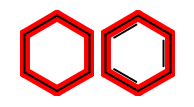
\includegraphics{benzene_cyclohexane_map.png}
    \caption{An example of an apparently reasonable atom map between benzene and cyclohexane.
    }
    \label{fig:benzene_cyclohexane_map}
\end{figure}
%
\begin{figure}
    \centering
    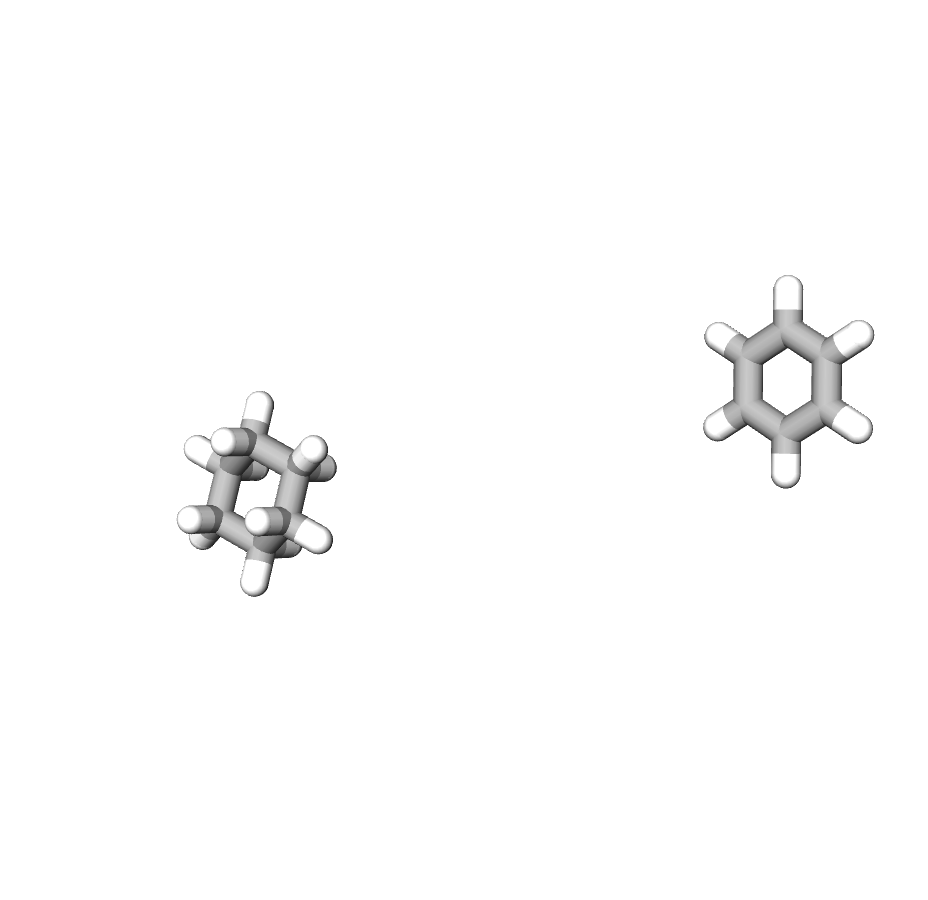
\includegraphics[width=1.0\textwidth]{cyclohex_ben_3d.png}
    \caption{3D structures of benzene and cyclohexane. Note that benzene is flat, while cyclohexane adopts a "chair" conformation.}
    \label{fig:benzene_cyclohexane_3D}
\end{figure}
%
To illustrate the consequence of improper atom maps (for instance, that disregard bond order), note Figure~\ref{fig:badbondorder}.
%
\begin{figure}
    \centering
    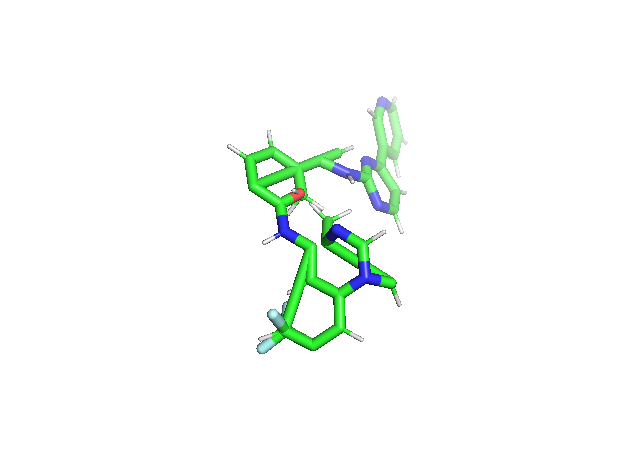
\includegraphics[width=1.0\textwidth]{failed_ring.png}
    \caption{A geometry that was constructed from an atom map that left no space to properly close the rings.}
    \label{fig:badbondorder}
\end{figure}
%
The simple inclusion of the bond order as a criterion for atom mapping greatly enhances the geometry that is produced, as in Figure~\ref{fig:goodbondorder}
%
\begin{figure}
    \centering
    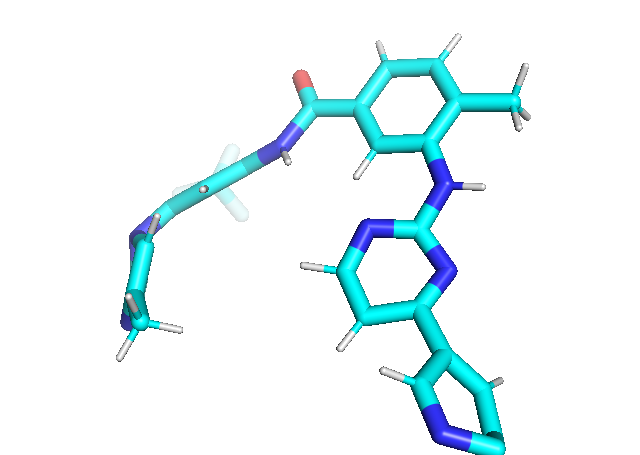
\includegraphics[width=1.0\textwidth]{success_ring_closure.png}
    \caption{A geometry resulting from the inclusion of bond order as a criterion for mapping atoms. More of the system is rebuilt, so a better geometry can be created.}
    \label{fig:goodbondorder}
\end{figure}
%
\section{Factors that affect acceptance probability}
%
For example, in Figure~\ref{fig:benzene_cyclohexane_map}, there are two molecules with six-membered carbon rings.
%
Mapping these would seem intuitive based on graph structure, but the nature of the edges makes this prohibitively unfavorable.
%
The 3D structures of these molecules, visualized in Figure~\ref{fig:benzene_cyclohexane_3D}, demonstrate that this is highly infeasible---the initial structure of either will be very unfavorable using the potential of the other.
%
In this case, chemical intuition would make the problem obvious: benzene is aromatic, while cyclohexane is not.
%
In many other cases, the distinction may not be clearly obvious.
%
\begin{figure}[h]
    \centering
    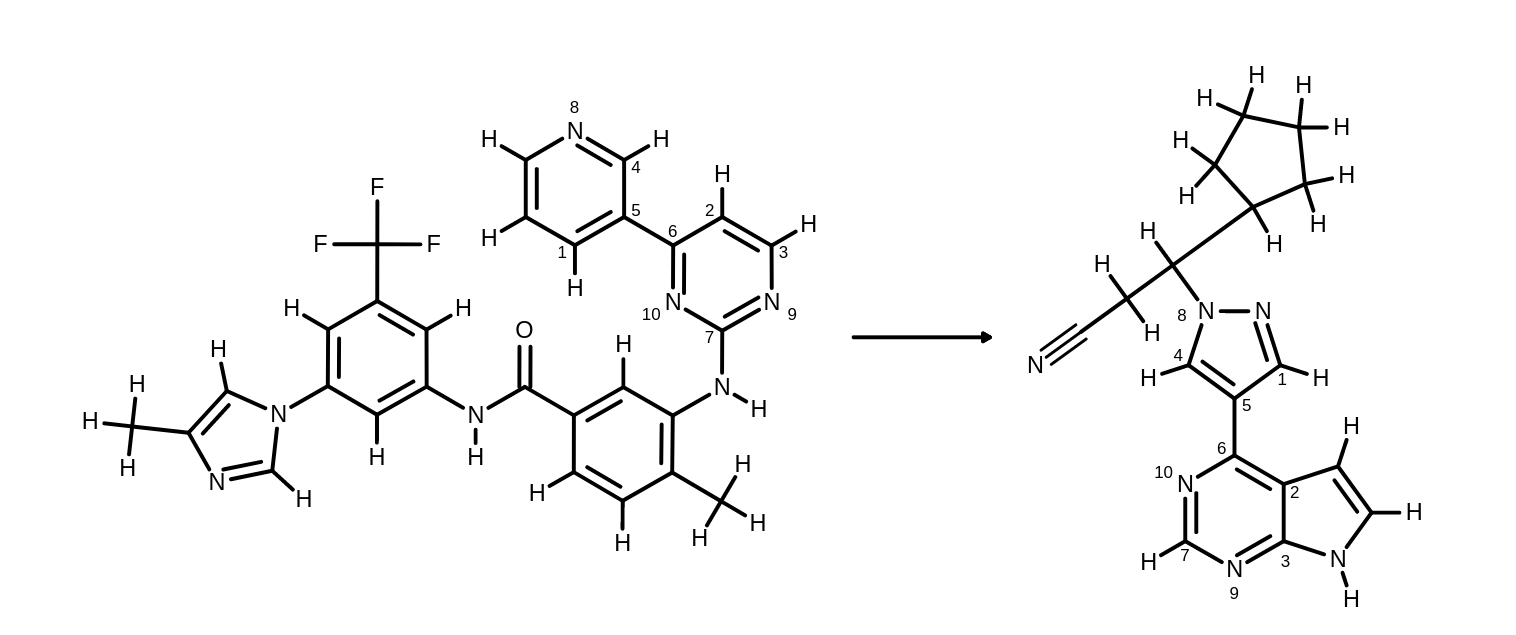
\includegraphics[width=1.0\textwidth]{kinase_map_bad.png}
    \caption{This map between kinase inhibitors may contain more atoms than another, but as it is partially breaking a ring, energies after the proposal are often highly unfavorable}
    \label{fig:bad_kinase_map}
\end{figure}
%
In Figure~\ref{fig:bad_kinase_map}, we see an example of the MCSS algorithm maximizing the overlap between two molecules in terms of the atom map.
%
However, it may be naive to attempt this, as the dimension-matching component of the algorithm will now have to complete the ring, and the annealing will have to gradually introduce part of the ring.
%
In this instance, the random choice of atom maps would be helpful, as the algorithm would occasionally not choose the ring-breaking map.
%
An attractive alternative to randomly choosing an atom map is to simply filter out maps that partially map rings.
%
While the toolkit that I used for this project unfortunately did not provide this as an option, it is possible to simply eliminate the maps that break rings.
%
The algorithm for determining whether rings are broken is as follows, with a return value of True signifying that rings are broken:
%
\begin{itemize}
    \item For a pair of molecules $(k, k')$, enumerate the cycle basis of both molecular graphs~\cite{paton1969algorithm}
    \item For each bond in a cycle of molecular graph $k$, check that it is in graph $k'$, if any are not, return True
    \item If all bonds in cycles of $k$ are also in $k'$, return False
\end{itemize}
%
This algorithm checks that rings are not created or destroyed, and is done using the NetworkX toolkit~\cite{Hagberg2008}.
%
However, building an entire ring is not infeasible, and so the algorithm could be modified to check that if a ring is created or broken, an entire ring is created or broken.
%
\subsection{An exploration of the effect of various atom mapping options on acceptance probability}
%
As an interesting exploration, I measured the empirical effect of different atom mappings on the variance of the instantaneous acceptance probabilities between various substituted benzene molecules as shown in Figure~\ref{fig:substituded_benzene_maps}.
%
\begin{figure}
    \centering
    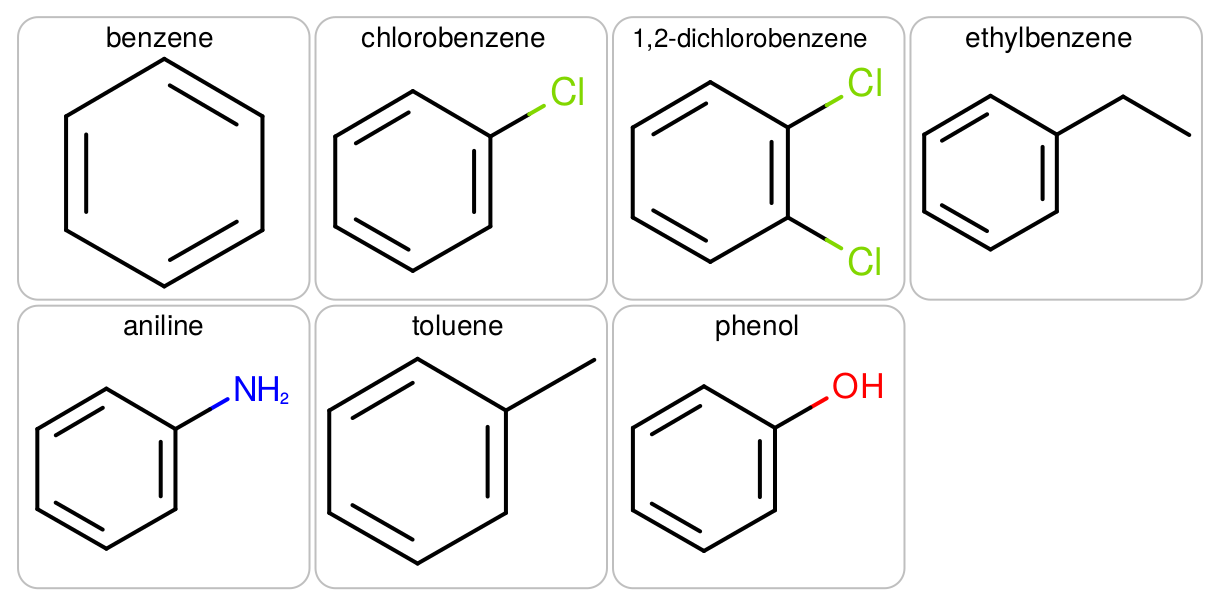
\includegraphics[width=0.5\textwidth]{mol_atom_map.png}
    \caption{The set of trial molecules used for empirical exploration of atom map criteria. This set was used to demonstrate because it contains very similar cores, but different substituents that might affect the performance of atom maps.
    }
    \label{fig:substituded_benzene_maps}
\end{figure}
%
In this experiment, I ran the molecules at a timestep of 1 femtosecond for 1 nanosecond at 300 Kelvin in vacuum, taking a snapshot of the trajectory every picosecond.
%
For each other molecule in the set, I attempted 100 reversible jump proposals under each atom matching scheme, starting from a configuration randomly drawn from the equilibrium cache of the starting molecule.
%
As is readily apparent from Figure~\ref{fig:benz_chlorobenz_different_maps}, the choice of map can have a significant effect on the quality of the proposal.
%
\begin{figure}
    \centering
    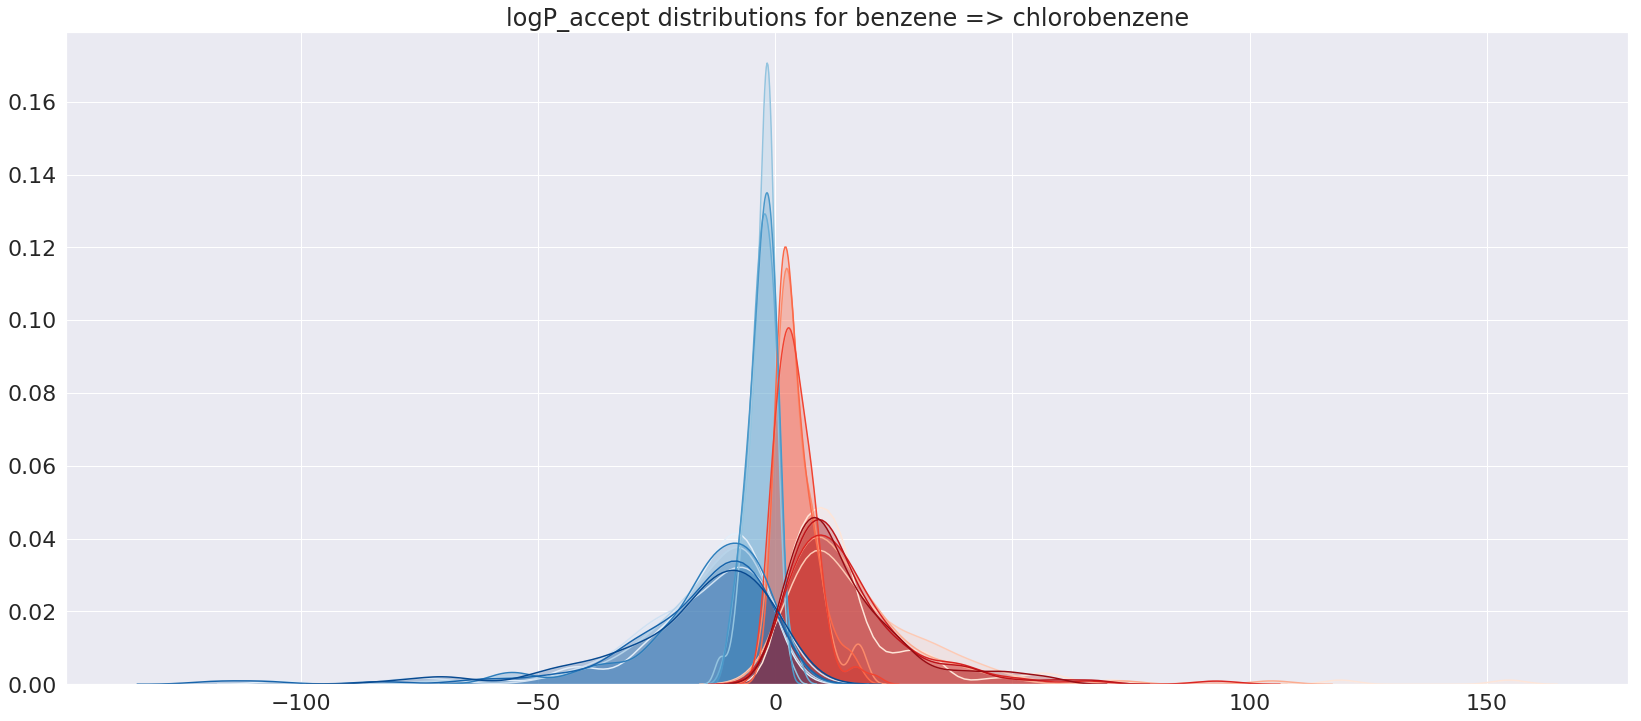
\includegraphics[width=\textwidth]{benzene_chlorobenzene_maps.png}
    \caption{Forward (blue) and negative reverse (red) log acceptance probability distributions for benzene to chlorobenzene in vacuum under different mapping schemes. Here, it is clearly visible that the choice of mapping scheme has a profound effect on the ultimate quality of the proposal.}
    \label{fig:benz_chlorobenz_different_maps}
\end{figure}
%
However, for some other pairs, the choice of map does not appear as important.
%
For example, in Figure~\ref{fig:toluene_phenol_different_maps}, the various maps produce distributions of acceptance probabilities that cluster around the the same region.
%
As such, it is an area of active investigation to determine how to map atoms in a way that maximizes the efficiency of the computation.
%
\begin{figure}
    \centering
    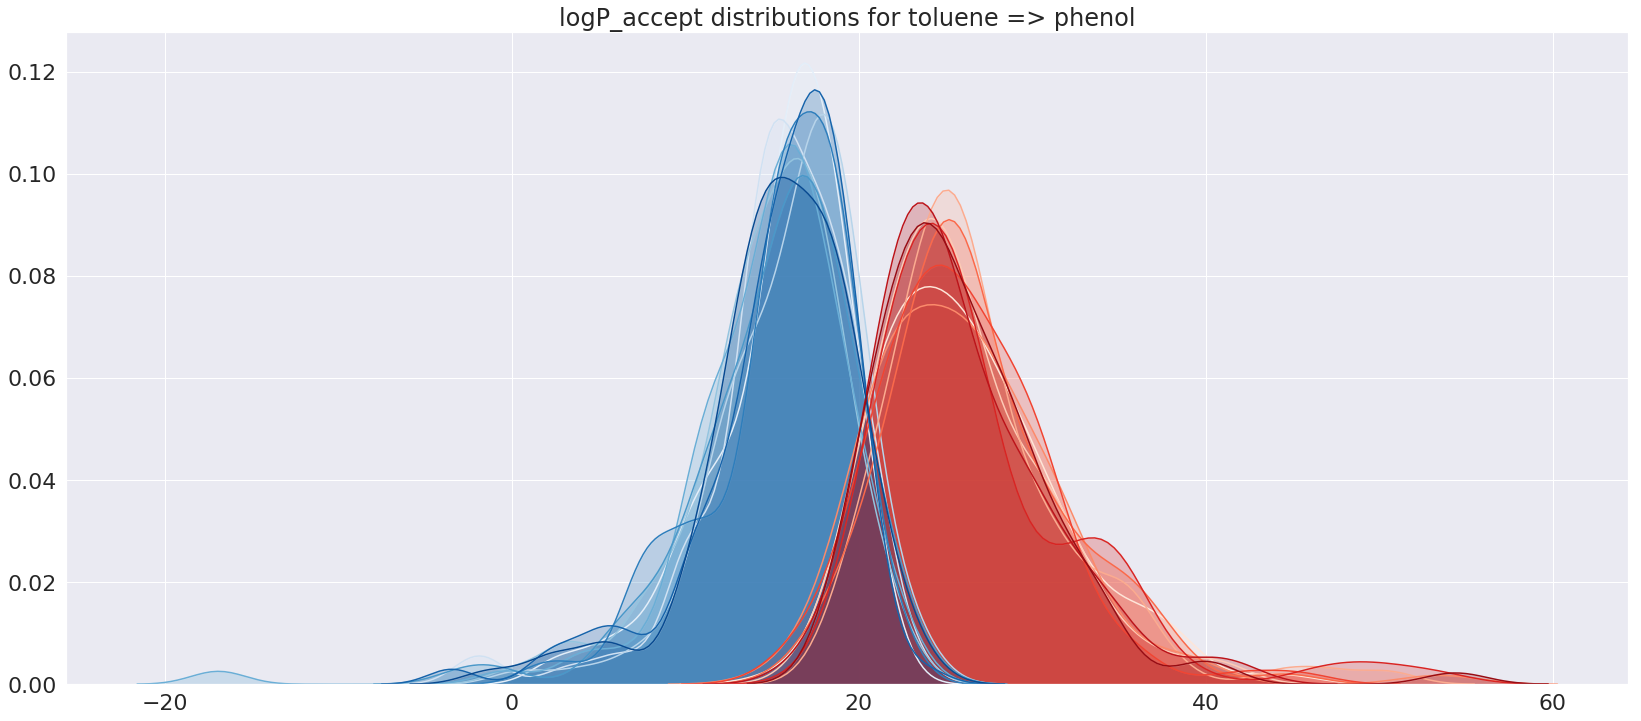
\includegraphics[width=\textwidth]{toluene_phenol_maps.png}
    \caption{Forward (blue) and negative reverse (red) log acceptance probability distributions for toluene to phenol in vacuum under different mapping schemes. Here, the choice of the mapping scheme does not seem to have as significant of an impact on the quality of the proposal.}
    \label{fig:toluene_phenol_different_maps}
\end{figure}
%
It is clearly of interest in practical applications to understand what the ideal atom mapping criterion for explicit solvent is, and whether this differs substantially from the criteria chosen in vacuum.
%
\section{Future work}
%
\subsection{Atom map learning}
For OpenEye MCSS, there are multiple atom map options.
%
For instance, the user can choose to have the MCSS algorithm match atoms based on aromaticity, element, number of heavy bond partners, and more.
%
In principle, these discrete choices can be enumerated and searched to find near-optimal combinations
%
This does leave open the question of what to use as the objective.
%
In principle, the variance of the acceptance probability is ideal, though it may be difficult to estimate.
%
Alternatively, one could try to find the set of discrete hyperparameters that maximize the average acceptance probability, which is straightforward to compute.
%
This does, however, leave the issue that a set of atom mapping parameters ideal for one set of molecules may not be performant for another.
%
\subsubsection{Treat atom mapping as a Reinforcement Learning problem}
%
As a result, one could imagine treating the atom mapping as a reinforcement learning problem, wherein an agent must select a set of parameters given the transformation at hand~\cite{Sutton1988, Watkins1992}.
%
In this way, one might hope that the algorithm could learn general rules that would be valid across many different sets of molecules.
%
One advantage of this approach is that, under certain conditions~\cite{Andrieu2005, Andrieu2007, Andrieu2008}, one could potentially design an adaptive MCMC algorithm that performs this learning as the calculation proceeds.
%
This would potentially allow the user to avoid a costly pre-optimization (or the use of suboptimal parameters derived from a reference set).
%
\subsubsection{Atom mapping with neural network}
%
Finally, one might also simply leave the atom mapping choice to a neural network, leaving open the possibility to efficiently learn a function mapping from transformations (or even environments) to atom maps.
%
Although the map itself is discrete, other sophisticated differentiable neural architectures such as the differentiable Forth interpreter~\cite{bosnjak17} were able to overcome this.
%
\subsection{Relieving the restriction to a finite set of chemicals}
%
Ideally, the simulation would not be limited to a prespecified set of chemical states.
%
Rather, one could imagine applying synthetic transformation rules to generate new, feasible chemicals.
%
This has the advantage of resulting in chemical matter that is more likely to be feasible to synthesize (or at least more likely to be able to convince a chemist to try).
%
Alternatively, one could imagine using an RNN such as in \cite{Gupta2017}, where a neural network might learn to generate new chemicals.
%
In this way, we might not only adaptively solve the issue of which chemical states are "neighboring," but also push toward synthetic novelty in a way that humans have not been able to.
%
Although there are challenges in this part of the algorithm, many of the challenges for expanding beyond a fixed set of chemical species lie in the weight adaptation algorithm, discussed later.
%
The development of this algorithm opens up new avenues for exploration, as well as new avenues for multidisciplinary collaboration with other fields.

\chapter{Geometry Proposals}

\section{Introduction to dimension matching}

Although Reversible Jump MCMC~\cite{GREEN1995} provides a very general and convenient framework for sampling spaces with varying dimensionality, there are still many practical and problem-specific considerations.
%
Neglecting other components of the acceptance probability, the contribution to the acceptance probability involving dimension matching in the proposal from $(x_{old}, k) \rightarrow (x_{new}, k')$ is given by

\begin{equation} \label{eq:geometry}
    \ln P_\mathrm{geometry} = \left[-u_{k'}(x_{new}) + u_{k}(x_{old})\right] + ln\frac{\phi (x_{old}~|~x_{new})}{\phi (x_{new}~|~x_{old})}
\end{equation}
%
where $u_{k'}$ is the reduced potential for chemical state $k'$, $u_k$ is the reduced potential for chemical state $k$, $x_{new}$ is the new proposed configuration, $x_{old}$ is the old configuration, and $\phi(x,y)$ is the dimension matching distribution.
%
Notably, $x_{new}$ and $x_{old}$ can have different dimensionalities.
%
Intuitively, this involves ensuring that the spaces on which the proposal and the current distribution lie are the same.
%
In other words, we must augment each probability distribution with another distribution that contributes the missing degrees of freedom for each.
%
However, although the recipe is in principle straightforward, it is difficult to construct an efficient dimension matching distribution for the case of chemical space sampling.
%
Among the challenges for constructing an efficient distribution are the multimodality of the target distribution, the need to draw an exact sample, and the need to be able to calculate a normalized probability for the proposal.
%
\section{Problems faced by dimension matching in chemical space}
%
\subsection{The target is highly multimodal}
%
Consider a flexible alkane: a terminal methyl group could be rotated to produce configurations of roughly even probability.
%
Although one might not consider this to be a significant problem, consider the terms in Eq.~\ref{eq:geometry}.
%
The positive contribution of the reverse proposal probability (that is, the probability of placing the atoms being deleted where they were found) means that the proposal distribution must not simply place atoms in a favorable position; it must also recognize favorable positions as such.
%
To use a more concrete example, consider the pair of distributions in Figure~\ref{fig:1D-geometry}. 
%
Although the proposal distribution would clearly place a sample in a favorable location, a sample drawn from the target (such as from a Langevin dynamics simulation) would likely have low probability under the proposal.
%
\begin{figure}[h]
    \centering
    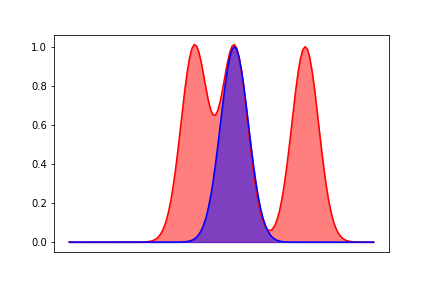
\includegraphics[width=1.0\textwidth]{unimodal.png}
    \caption{An example of a unimodal proposal (blue) with a multimodal target(red). Note that there are many regions of the target that are poorly covered by the proposal.}
    \label{fig:1D-geometry}
\end{figure}
%
This prevents algorithms that, for instance, use a single reference torsion for proposals.
%
As a result of these complex interactions and multimodal distributions, many simple sampling schemes are ruled out.
%
\subsection{The proposal must be drawn exactly}
%
Another choice that may seem attractive is to simply run an MCMC chain for the missing degrees of freedom and use that sample for the new coordinates.
%
However, in order for this to be drawn \emph{exactly} from the target distribution, the Markov chain would have to be run infinitely long (except in the case of perfect MCMC \cite{brooks2011handbook}, which is not applicable here).
%
This is clearly infeasible, and leaves us without familiar tools that we use to sample high-dimensional multimodal probability distributions.
%
\subsection{The proposal must be associated with a normalized probability}
%
Yet another temptation at this point may be to simply draw from a tractable distribution as in the Hastings algorithm~\cite{Hastings1970} (for example, a Gaussian), and then minimize the configuration's energy.
%
However, performing such a nonlinear transformation on the proposed configuration would require that we be able to invert and differentiate the transformation--the determininant of the Jacobian matrix of the transformation is required to calculate the probability.
%
Since we cannot straightforwardly compute such a Jacobian, techniques involving complex nonlinear transformations are largely impractical in this case.
%
\subsection{Atomic positions are correlated}
Further complicating the matter is the fact that various degrees of freedom in a molecule are correlated.
%
For instance, steric hindrance prevents atoms from being placed close to one another.
%
This means that although \emph{a priori} an atom might have a multimodal probability distribution, conditioned on a previous atom, some modes are now precluded.
%
\subsection{Propose one atom at a time}
%
Since proposing a set of atoms at once is fraught with difficulty as described above, one alternative is to propose one atom at a time, significantly reducing the dimensionality of the proposal distribution.
%
However, the challenges described above (especially multimodality and correlated atomic positions) still remain.
%
Following other literature in Grand Canonical Monte Carlo (GCMC) \cite{Siepmann1992} as well as in other molecular simulation literature and statistical literature~\cite{COMBE2003}, we propose positions in so-called internal coordinates.
%
In this coordinate system, atomic positions are defined by a bond length $r$, a bond angle $\theta$, and a dihedral angle $\phi$ as described in Figure~\ref{fig:internal}.
%
\begin{figure}
    \centering
    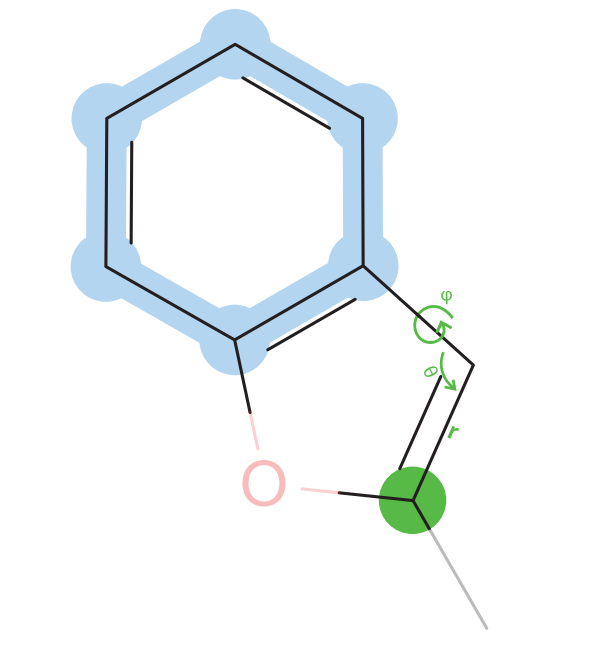
\includegraphics[width=0.4\textwidth]{internalcoords.png}
    \caption{An example of an internal coordinate description of atomic positions. The atom highlighted in green is being proposed, based on the bond (r), angle ($\theta$), and torsion ($\phi$).}
    \label{fig:internal}
\end{figure}
%
\subsection{Naive bond/angle/torsion doesn’t work}
%
Having moved to internal coordinates, the most obvious proposal scheme would be to choose a dihedral angle associated with each atom, and directly propose a bond length, bond angle, and dihedral angle based on the forcefield parameters.
%
However, this has a major pitfall: Although it works with simple geometries and cases where very few atoms need to be added, it fails quickly with complex geometries such as rings, as well as cases where many atoms must be added.
%
In the latter case, one can imagine that neglecting other dihedral and bond angle terms can easily lead to very unfavorable configurations for complex molecules.
%
As a refinement of this algorithm, we include other angle, dihedral, and even nonbonded terms in the proposal scheme.
%
\section{CBMC-like Algorithm}
%
For the common dimension-matching tasks, I implemented and refined a CBMC-like \cite{Siepmann1992, Andrieu2010pmcmc, COMBE2003} algorithm that can take into account forcefield terms besides one bond, angle, and torsion term. 
%
\subsection{Description of algorithm}
The CBMC-like algorithm with guide torsions has several components as follows.
%
At a high level, for a given transformation $k \longrightarrow k'$:
%
\begin{itemize}
    \item Determine which degrees of freedom, based on the atom map, are present in $k'$ not not $k$
    \item Separate atomic degrees of freedom into heavy atoms and hydrogens
    \item Perform a breadth-first search of the molecular graph, identifying the order in which heavy atoms can be proposed
    \item Repeat for hydrogen atoms
    \item For each new atom, propose a bond length, bond angle, and dihedral angle, and convert to cartesian coordinates
    \item Accumulate the log probability of the acceptance probability (described in detail below)
\end{itemize}
%
\subsubsection{Determining the atomic proposal order}
%
After determining which atoms are not mapped, the dimension-matching algorithm must first determine the order in which to propose the new atoms, as well as which internal frame of reference will be used.
%
In greater detail, beginning with a $\ln P_\mathrm{choice} = 0$, a set of atoms with positions and without positions, and until all new atoms are added:
\begin{itemize}
    \item Add atoms which do not have positions, but are connected to a bond, angle, and dihedral partner with positions to atoms\_eligible\_for\_proposal
    \item Uniformly choose without replacement atoms from the atoms\_eligible\_for\_proposal list, and add the probability of choosing each atom to $\ln P_\mathrm{choice}$
    \item For each atom that is chosen, uniformly choose a dihedral angle, and add the probability of this to $\ln P_\mathrm{choice}$
    \item Add each atom that is chosen to atoms\_with\_positions
\end{itemize}
%
The above algorithm is first conducted for the heavy atoms, and then for the hydrogens.
%
When the reverse proposal probability is being evaluated, the same procedure is repeated with stochasticity.
%
It is noteworthy to add here that the use of this algorithm for determining proposal order imposes an extra requirement on the atom map: it must contain at least one atom with a dihedral that can be used for proposal.
%
%
\subsubsection{Coordinate proposal algorithm}
%
Once the proposal order and the reference frame for each atom has been chosen, the algorithm can now stochastically propose coordinates for the new atoms.
%
For each new atom, along with its corresponding dihedral, the proposal algorithm works as follows:
%
\begin{itemize} \label{geometry_algorithm}
    \item If the bond is not constrained, propose bond length $r \sim p(r)=\mathcal{N}(r_0, \sigma^2_r)$, where $\mathcal{N}(\mu, \sigma^2)$ denotes the normal density with mean $\mu$ and variance $\sigma^2$, and $\sigma_r = (\beta K_r)^{-1/2}$ where $K_r$ is the bond force constant; if the bond is constrained, set $r$ to its constraint length $r_0$
    \item Propose bond angle $\theta \sim \mathcal{N}(\theta_0, \sigma^2_\theta)$, where $\sigma_\theta = (\beta K_\theta)^{-1/2}$, where $K_\theta$ is the angle force constant
    \item Propose dihedral angle $\phi \sim p(\phi; r, \theta)$, where $p(\phi ; r, \theta)$ is defined below
    \item Calculate $(x, y, z), \ln \det J(r, \theta, \phi) \longleftarrow$ internal\_to\_cartesian, where $J(r, \theta, \phi)$ is the Jacobian describing the hypervolume $dx \, dy \, dz$ given $dr \, d\theta \, d\phi$, where internal\_to\_cartesian converts from internal coordinates to cartesian coordinates.
    \item Compute the log contribution to the acceptance probability, $\ln P_\mathrm{atom} = \ln \left[ p(r) \, p(\theta) \, p(\phi; r, \theta) \, J(r, \theta, \phi) \right]$

\end{itemize}
%
Note that in Algorithm~\ref{geometry_algorithm}, we are able to use the forcefield's distribution (harmonic) for the bond and angle terms. 
%
However, the dihedral conditional density $p(\phi; r, \theta)$---in the absence of any other nonbonded interactions involving the placed atom---has the form
%
\begin{eqnarray}
p(\phi; r, \theta) &\propto& \exp\left[ -\beta \sum_{l=1}^L \frac{K_{\phi,l}}{2} cos(n_l \phi + \gamma_l) \right]
\end{eqnarray}
%
which does not have a closed-form normalizing constant; here, $K_{\phi,l}$ is a barrier height, $n_l$ is an integral periodicity, and $\gamma_l$ is a phase for the $l$th Fourier term.
%
It is straightforward to numerically normalize this, however, and draw samples using rejection sampling, since the distribution is only one dimensional.
%
Simply drawing from the conditional dihedral term is attractive, but generally affords poor performance, as it neglects most other terms.
%
For linear alkanes and small additions, this approach is feasible.
%
However, for more complex molecules, this approach suffers from several drawbacks. 
%
First, it neglects other valence terms such as the other dihedrals and angles in which the atom in question is involved.
%
Second, it will very often fail to properly create rings, since without the full set of bonds, intermediate dihedral angles would be just as likely to leave the ring open, causing extremely unfavorable valence interactions.
%
Finally, it does not afford the dimension matching scheme an opportunity to incorporate local nonbonded terms.
%
\subsubsection{Improvements to dihedral proposal density}
%
Rather than simply normalizing a single dihedral term and proposing from that, one can instead perform a drive of the angle about its dihedral, and compute the potential energy at each point.
%
This potential may be the full potential, or, for efficiency reasons, a subset of the full potential.
%
Then, having performed the dihedral scan, one can normalize the resulting potential to form a proposal density.
%
An additional hyperparameter of this algorithm is how finely discretized the dihedral angles must be.
%
\subsection{Performance on simple cases}
%
There are a number of different transformations that could be examined.
%
\subsubsection{Substituted Benzenes}
%
Among the simplest are transformations between different substituted benzenes as shown in Figure~\ref{fig:sub_benz}
%
These transformations are straightforward since the molecules are fairly rigid, and there are only several atoms to insert.
%
\begin{figure}
    \centering
    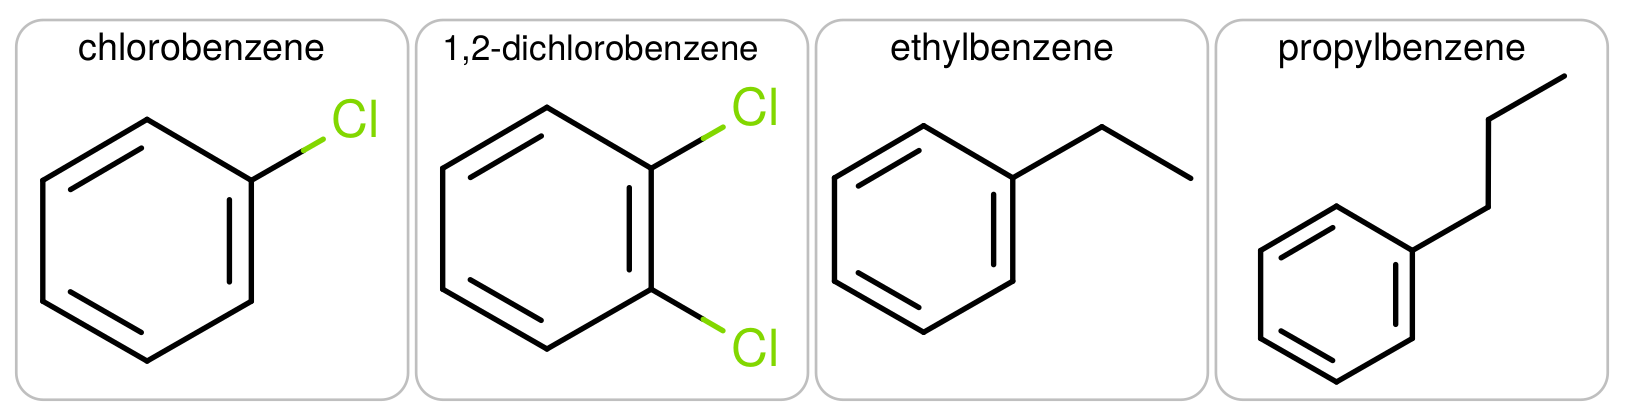
\includegraphics[width=1.0\textwidth]{subs_benz.png}
    \caption{Examples of substituted benzenes}
    \label{fig:sub_benz}
\end{figure}
%
\subsubsection{Alkanes}
%
Another type of transformation that is relatively straightforward is that between alkanes, as shown in Figure~\ref{fig:n-alkanes}.
%
However, these molecules are more flexible, and thus the dimension matching distribution must accurately capture the multimodality of the configurational probability distribution.
%
\begin{figure}
    \centering
    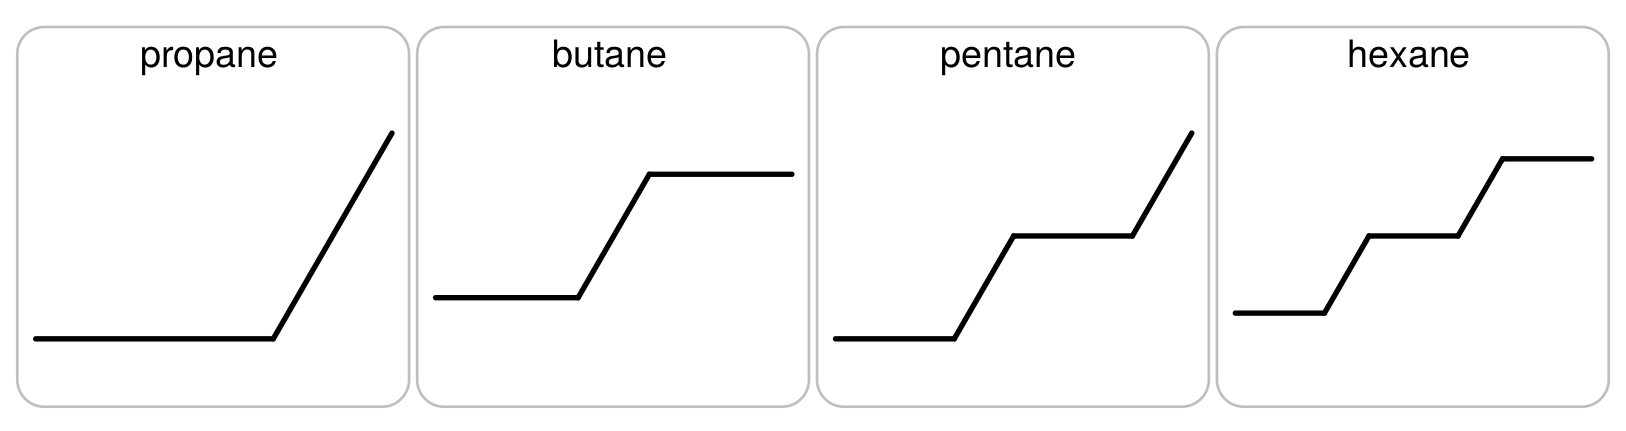
\includegraphics[width=1.0\textwidth]{alkanes.png}
    \caption{Examples of n-alkanes}
    \label{fig:n-alkanes}
\end{figure}
%
\subsubsection{More complex transformations}
%
Of course, while alkanes and substituted benzenes are useful model systems and the building blocks of many interesting compounds, we are far more interested in complex transformations, such as the addition of rings or jump between different drug-like molecules.
%
In order to achieve these, however, we must further improve our strategy.
%
One immediate difficulty, even with the improved dihedral scan, is that building a ring will often result in failure.
%
The failure to close a ring results from the fact that when the intermediate ring atoms are being inserted, there are no terms that cause the ring to close, resulting in a grotesque geometry.
%
To remedy this, we can add "guide torsions" that encourage the ring to close by removing the dihedral modes that correspond to an open ring as in~\cite{Wick2000}.
%
The algorithm for the addition of guide torsions works as follows:
\begin{itemize} \label{ringclosure}
    \item Convert the molecule into the OpenEye OEMol format
    \item Perceive rigid bonds
    \item Generate a reference configuration using OpenEye Omega
    \item Measure the dihedral angles about the rigid bonds
    \item Add a dihedral term with a mode at the angle in the reference conformation
\end{itemize}
%
By applying the steps in Algorithm~\ref{ringclosure}, we can significantly increase the chance of proposing a closed ring, resulting in a more realistic geometry.
%
\subsection{Shortcomings}
%
However, with very large changes (involving the addition of many atoms), this approach is still not terribly performant.
%
As an example of Sequential Importance Sampling (SIS), it suffers from the compounding of poor choices made earlier in the sequence.
%
As the number of degrees of freedom that must be added grows, this problem becomes more serious, demonstrated in Figure~\ref{fig:dof_added_worse}.
%
\begin{figure}
    \centering
    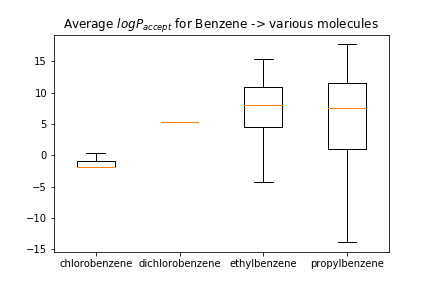
\includegraphics{dof_demo.png}
    \caption{The average $\ln P_\mathrm{accept}$ \emph{vs.} the number of degrees of freedom added. 
    Note that the variance is quite low for small (chlorobenzene and dichlorobenzene) changes, but quickly grows with the addition of flexible chains. Note that anything beyond the 98th percentile was clipped for this figure.}
    \label{fig:dof_added_worse}
\end{figure}
%
When the approach is tried on even more complex transformations, such as between kinase inhibitors, we observe even more severe performance loss, making acceptance a highly unlikely proposition.
%
However, there are yet remedies to these serious problems.
%
\section{Future directions: Particle Filtering}
%
\subsection{Basic Overview}
%
Instead of simply choosing one dihedral angle at each atom in \ref{geometry_algorithm}, we can choose N dihedral angles and calculate an importance weight based on the difference between the probability of that atom's placement under the target distribution.
%
Then, after a specified number of atoms are inserted, the algorithm resamples $N$ of the configurations based on their weights.
%
This technique is called particle filtering \cite{DelMoral1997,Henriksen2012}, and is commonly used in state space models.
%
\subsection{Advantages}
%
Particle filtering can enable the algorithm to eliminate proposals that were reasonable at stage $m$ but become very unfavorable at stage $m+n$.
%
For example, if a “particle” (as the replicates of configurations are known in statistics) does not close a ring, when the ring closure should happen, its weight will be very small and it will be lost in the resampling.
%
On the other hand, naive multinomial resampling carries with it its own risks: since at every resampling step there is a nonzero probability for favorable configurations to be lost, after enough resampling steps, the probability that favorable configurations are lost can grow quite high.
%
Mitigating this are other resampling algorithms, which aim to reduce the deleterious effect of multinomial sampling
%
In addition to these advantages, particle filtering can be parallelized on tightly-coupled parallel hardware such as graphics processors~\cite{lee2010utility}.
%
\subsection{Algorithm Hyperparameters}
%
As briefly mentioned above, the particle filter has a number of hyperparameters that can be tuned and tweaked.
%
Among these are the number of particles or replicates, the method used for resampling, and, as above, the method used for proposing the individual bonds, angles, and dihedrals. 
%
\subsubsection{Number of Particles}
The most obvious algorithm hyperparameter is the number of particles. The larger this number is, the better the performance of the dimension matching algorithm.
%
However, each particle requires the computation of the target density, which can be quite expensive.
%
Because cost scales relatively quickly in this case, it would be ideal to minimize the number of particles needed.
%
Furthermore, a very large number of particles can cause serious numerical instabilities \cite{Murray2016}, primarily from the need to normalize weights before resampling.
%
\subsubsection{Resampling Algorithm}
One can choose various approaches for the resampling step of the particle filter. 
%
The simplest is known as multinomial resampling, and consists of simply drawing $N$ particles with replacement from the previous $N$ according to their weights.
%
This is known to have a relatively high variance \cite{Douc2005}.
%
Another approach is so-called stratified resampling, which 
%
This also requires weight normalization, however.
%
In situations with large numbers of particles, it may be feasible to resort to a scheme that is "almost" exact, such as Metropolis resampling. \cite{Murray2016}
%
In the Metropolis resampling scheme, one proposes to sample a particular ancestor and accepts/rejects.
%
One then repeats this procedure many times until approximate convergence.
%
These steps must be performed at each resampling attempt.
%
This is not technically exact, as Metropolis MCMC only converges in the asymptotic limit, not for finite samples.
%
However, in some studies \cite{Murray2016}, it actually has less bias than the exact methods, because weight normalization is not required and certain numerical issues are resolved
%
Parallelization is also facilitated by Metropolis resampling, since the weights do not need to be normalized (a reduction operation) before resampling.
%
\subsubsection{Overall comparison}
Finally, below is a table which compares the features of various proposal schemes that are in principle correct for the dimension matching algorithm.
%
\begin{table}
\caption{{\bf Comparison of features of various proposal schemes for dimension matching.}
\label{tab:proposal-scheme-comparison}
}
\begin{center}
    \footnotesize
    \begin{tabular}{||c | c | c | c | c | c | c||}
    \hline
         Method & Multimodal & Exact & computable P & Rings & Correlated & Speed \\
         \hline
         Minimization &  Yes & Yes & No & Yes & Yes & Fast \\
         Unimodal & No & Yes & Yes & No & No & Fast \\
         Multi-reference & Yes & Yes & Yes & Yes & No & Fast \\
         CBMC-like & Yes & Yes & Yes & No & Moderate & Moderate \\
         CBMC+guide & Yes & Yes & Yes & Yes & Moderate & Moderate\\
         Particle Filtering & Yes & Yes & Yes & Yes & Yes & Slow \\
         \hline
    \end{tabular}
\end{center}
\end{table}
%
%
\section{Tuning of Dimension Matching Parameters in the context of NCMC}
%
It should be noted that although the parameters for the dimension matching proposal are very important, there are several tradeoffs between tuning the parameters of the dimension matching and those of the NCMC or annealing, described in the next chapter.
%
The implementation details of each are quite different, leading to interesting tradeoffs.
%
For instance, although the energy computations in the dimension matching algorithm are much faster (they exclude the majority of the system's interactions), the annealing runs on the GPU, which often more than compensates for the added terms in the energy computation.
%
An additional point to note is that the dimension matching (especially particle filtering) can be subject to numerical stability issues.
%
Because the annealing protocol is typically very slow, and steps of Langevin Dynamics are taken between changes in the control parameter, the NCMC component of the overall algorithm may be better behaved.
%
For this reason, it is useful to jointly optimize the parameters.
%
\subsection{Tradeoffs}
%
There is to some extent a tradeoff between the hyperparameters of the dimension matching algorithm, and those of the annealing.
%
Intuitively, one might imagine that additional grid points and the use of nonbonded forces in the dimension matching scheme might result in the need for fewer steps of NCMC.
%
However, due to the current setup of the NCMC, this is not terribly helpful.
%
Nonbonded forces are initially disabled for the new atoms (except intramolecular nonbonded forces), and so using the constributions of intermolecular nonbonded forces to proposed new geometries is likely to result in an inferior acceptance probability.
%
As to the number of grid points, this could potentially be reduced with longer NCMC by including valence softening in the NCMC.
%
However, the default configuration of NCMC does not include this, and so the number of grid points is largely decoupled from the NCMC protocol length.
%
However, another potentially fruitful approach is to allow the NCMC code to soften the bonds and angles at the initial value of the control parameter.
%
This allows otherwise unfavorable geometry proposals to be accorded a favorable energy, then slowly anneal back to the forcefield's parameters for those terms.
%
It should be noted that doing this would then introduce a dependency between the geometry proposal's hyperparameters and the NCMC protocol.
%
For example, it may result in the need for longer protocols, or may cause very unfavorable reverse geometry proposal probabilities.
%
To understand the latter point, consider that if the NCMC protocol is symmetric, the atoms to be deleted will conclude the protocol with soft bonds and angles, thus distorting the geometry from what the forcefield would otherwise cause.
%
However, the geometry proposal distribution is simply using the forcefield's parameters, and as such will likely assign low probability to the ending configuration.
%
This can be straightforwardly ameliorated by modifying the geometry engine to also be able to soften its bond and angle proposal distributions, thereby once again matching the distribution seen in the nonequilibrium switching.



\chapter{NCMC Switching}

\section{Introduction}
%
If new atoms are introduced into a condensed-phase simulation, it is highly likely that they will be placed unfavorably close to other atoms.
%
Additionally, if a ligand is transforming to another ligand, valence and nonbonded terms may also need to transform, as demonstrated in Figure~\ref{fig:benz_chlorobenz}
%
In order to mitigate these very serious issues, we turn to Nonequilibrium Candidate Monte Carlo (NCMC)~\cite{Nilmeier2011}. 
%
NCMC is a technique that allows us to gradually interpolate the system from one set of control parameters to another.
%
In this particular case, atoms are introduced after dimension matching as non-interacting dummies, and core atoms are left with their original parameters.
%
Then, the algorithm alternates between incrementing the control parameters and taking one step of Langevin dynamics (or other MCMC algorithm that either maintains the invariant distribution, or accounts for deviations by including an importance weight)
%
This allows new atoms to be introduced smoothly, and allows core atoms to be smoothly interpolated from one set of parameters to another.
%
\begin{figure}[H]
    \centering
    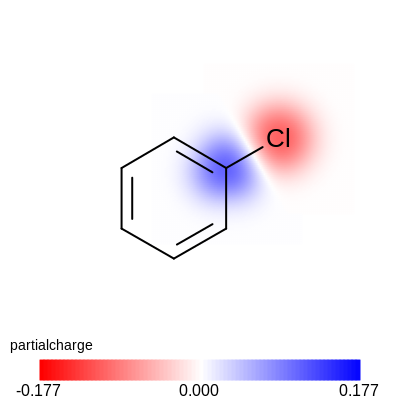
\includegraphics[width=0.5\textwidth]{partialcharge-pm.png}
    \caption{Chlorobenzene, with atoms colored by charge. If the ring is mapped to benzene (where all partial charges are equal), the abrupt change is very unfavorable.}
    \label{fig:benz_chlorobenz}
\end{figure}
%
\section{Description of Algorithm}
%
In broad terms, the algorithm performs the following steps:
\begin{itemize}
    \item Given system A, system B, and an atom map between them, generate hybrid system H with control parameters $\lambda \in [0,1]$
    \item Perform annealing or nonequilibrium switching, changing control parameters from 0 to 1 gradually and accumulating the change in energy
    \item Transfer the positions to system B
\end{itemize}
%
\subsection{Construction of Hybrid System}
%
The first step is to construct a system that is the hybrid of the two endpoints.
%
The object of constructing this system is to be able to smoothly interpolate from the first endpoint to the second.
%
To that end, I build the system with modified energy terms: all of the terms are controllable through global parameters collectively known as $\lambda$.
%
When $\lambda=0$, the hybrid system behaves like the initial endpoint.
%
When $\lambda=1$, the hybrid system behaves like the final endpoint.
%
The construction of such a system, as well as the path that one takes through the space of control parameters, are important factors in the performance of the overall algorithm.
%
Here, I will describe in greater detail the way that each type of energy term for a classical forcefield is handled.
%
\subsubsection{Bond force}
%
In the AMBER forcefields~\cite{Ponder2003}, bond forces are represented by a harmonic term:
%
\begin{equation} \label{eq:bondforce}
    U(r) = \frac{K_r}{2}(r - r_0)^2
\end{equation}
\noindent where the $K$ is a force constant and the $r_0$ is the equilibrium bond length. 
%
For bonds present in both endpoint systems in the region of the system that is being modified, I use a slightly modified potential:
\begin{eqnarray} \label{harmonic_alchemical}
    r_0 (\lambda_{bonds}) = (1 - \lambda_\mathrm{bonds}) r_{0_A} + \lambda_\mathrm{bonds} r_{0_B} \\
    K_r (\lambda_{bonds}) = (1 - \lambda_\mathrm{bonds}) K_{r,A} + \lambda_\mathrm{bonds} K_{r,B} \\
    U(r; \lambda_{bonds}) = \frac{K_{r} (\lambda_\mathrm{bonds})} {2} \left[ r - r_0(\lambda_\mathrm{bonds}) \right]^2
\end{eqnarray}
%
\noindent In this way, the hybrid system's bond energy linearly depends on the control parameter $\lambda_{bonds}$ between the endpoints.
%
We are also free to change the bond parameters nonlinearly with the master $\lambda$ control parameter's schedule.
%
For bonds that are not in the modified region, a standard harmonic term is used. 
%
Likewise, for bonds between atoms that only exist in one endpoint or the other, a standard harmonic term is used to prevent them from departing the region where they belong.
%
A tricky issue arises when two atoms are present in both systems, but have a bond only in one.
%
This arises in the case of transforming a non-ring into a ring.
%
In this case, for the system without the ring, the bond force constant is set to 0. 
%
However, it should be noted that these proposals are likely not desirable, and should be remedied by reducing the number of atoms in the map.
%
Finally, it is important to mention that when a constrained bond is encountered, its constraint length is not changed.
%
This is to avoid the need to compute a Jacobian for this deterministic transformation, although it would in principle be possible.
%
I have found that this issue can generally be avoided entirely by simply not mapping hydrogen atoms.
%
\subsubsection{Angle force}
%
Also included in AMBER force fields (as well as others) are angle terms between 3 atoms.
%
These force terms are also harmonic, with the form:
%
\begin{equation} \label{eq:angleforce}
    U(r) = \frac{K_{\theta}}{2}(\theta - \theta_0)^2
\end{equation}
%
I treat these similarly to the bonds in \ref{harmonic_alchemical}:
%
\begin{eqnarray} \label{harmonic_alchemical_angles}
    \theta_0 (\lambda_{angles}) = (1 - \lambda_\mathrm{angles}) \theta_{0_A} + \lambda_\mathrm{angles} \theta_{0_B} \\
    K_\theta (\lambda_{angles}) = (1 - \lambda_\mathrm{angles}) K_{\theta,A} + \lambda_\mathrm{angles} K_{\theta,B} \\
    U(\theta; \lambda_{angles}) = \frac{K_\theta (\lambda_{angles})} {2}\left[\theta - \theta_0(\lambda_{angles})\right]^2
\end{eqnarray}
%
As with the bonds, I do not use the modified potential for angles that are not in the region being modified, nor do I use them for triplets of atoms that are only present in one endpoint.
%
The ring closure issue is also present with the angles, and is handled similarly.
%
\subsubsection{Dihedral force}
%
Dihedral angles also have potential terms, of the form:
%
\begin{equation}
    U(\phi) = \sum_{l=1}^L \frac{K_{\phi,l}}{2} \cos(n_l \phi - \gamma_l)
\end{equation}
%
\noindent where $\phi$ is the dihedral angle, and for Fourier component $l \in \{1, \ldots, L\}$, $n_l$ is the periodicity, $\gamma_l$ is the phase, and $K_{\phi,l}$ is the force constant.
%
For the dihedrals present in both systems, I make the total energy a linear combination of the endpoint terms, dependent on a control parameter $\lambda_\mathrm{torsions}$:
%
\begin{eqnarray}
    U(\phi; \lambda_\mathrm{torsions}) = (1 - \lambda_\mathrm{torsions}) U_A(\phi) + \lambda_\mathrm{torsions} U_B(\phi)
\end{eqnarray}
%
Similarly to other valence terms, dihedral terms that are between atoms solely in one endpoint are always active to prevent very unfavorable configurations from being reached.
%
\subsubsection{Nonbonded terms}
%
Perhaps most challenging of all the energy terms are the nonbonded terms. Not only is there a great diversity of schemes for implementing long-range nonbonded interactions, but these parameters can have a very profound impact on the acceptance probability.
%
The nonbonded interactions of the AMBER~\cite{Ponder2003} forcefield consist of two components: electrostatics and Lennard-Jones or sterics.
%
The sterics component is a relatively short-range component with a form:
\begin{equation}
    U(r) = 4\epsilon\left[ \left(\frac{\sigma}{r}\right)^{12} - \left(\frac{\sigma}{r}\right)^6\right]
\end{equation}
%
\noident where $\epsilon$ is the depth of the potential well (how favorable it is to be in the minimum energy configuration) and $\sigma$ is the distance between the atoms where that minimum is located.
%
The electrostatics component is long-ranged and takes the form of the Coulomb force:
%
\begin{equation}
    U(r) = \frac{1}{4\pi\epsilon_0} \frac{q_i q_j}{r}
\end{equation}
%
\noindent where $q_i q_j$ is the product of individual atomic partial charges and $\epsilon_0$ is the vacuum permittivity.
%
Although initially one might be tempted to simply linearly interpolate the nonbonded terms, there is an immediate issue: although the sterics provide a repulsive term as two atoms become very close, the electrostatics term will (if the charges are of opposite sign) provide greater and greater attraction, leading to a singularity.
%
As such, I decouple the sterics and electrostatics interpolation so that there are six control parameters for the transformation of nonbonded terms: $\lambda_\mathrm{stericsdelete}, \lambda_\mathrm{stericsinsert}, \lambda_\mathrm{electrostaticsdelete}, \lambda_\mathrm{electrostaticsinsert}$, as well as two additional parameters, $\lambda_\mathrm{sterics}, \lambda_\mathrm{electrostatics}$ for core atoms whose identity is changing but are not being inserted or deleted.
%
Having divided up the control parameters as such, I then interpolate as in Figure~\ref{fig:nb_interpolation}.
%
%
\begin{figure}
    \centering
    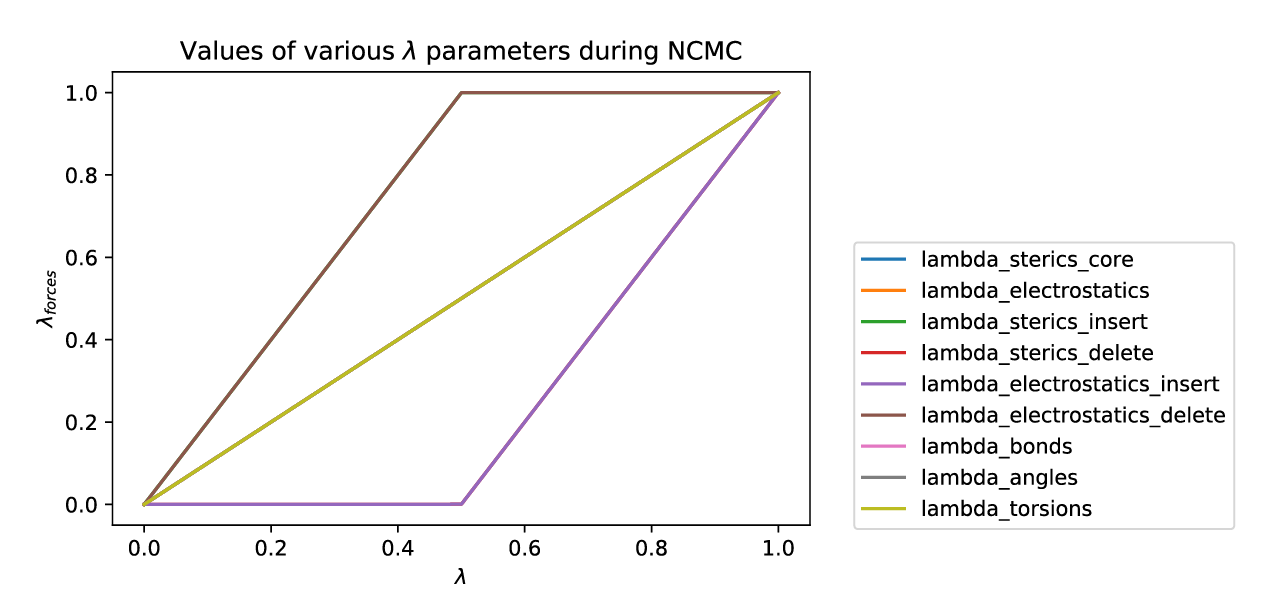
\includegraphics[width=0.8\textwidth]{lambda_traj_plotvec2-fixed.png}
    \caption{Nonbonded interpolation scheme, with the schedule of each individual force's $\lambda$ parameter plotted against the global $\lambda$. Note that sterics are always eliminated after electrostatics, and are always added before electrostatics. This provides protection against unshielded charges.}
    \label{fig:nb_interpolation}
\end{figure}
%
\subsubsection{Softcore sterics}
%
In order to provide greater simulation stability, I also utilize softcore sterics~\cite{Hornak2004}.
%
In this form, the sterics potential becomes:
\begin{eqnarray}
    U(r; \lambda_\mathrm{sterics}) &=& 4\epsilon\left[ \left(\frac{\sigma}{r}\right)^{12} - \left(\frac{\sigma}{r}\right)^6\right] \\
    \lambda_{\alpha} &=& \mathrm{dummy}_A (1-\lambda_\mathrm{sterics}) + \mathrm{dummy}_B (\lambda_{sterics}) \\
    \epsilon &=& (1 - \lambda_\mathrm{sterics}) \epsilon_A + \lambda_\mathrm{sterics} \epsilon_B \\
    \sigma &=& (1 - \lambda_\mathrm{sterics}) \sigma_A + \lambda_\mathrm{sterics} \sigma_B \\
    r_\mathrm{eff} &=& \sigma * \left[\alpha \lambda_\mathrm{sterics} (1 - \lambda_\mathrm{sterics}) + \left(\frac{r}{\sigma}\right)^6\right]^{1/6}
\end{eqnarray}
%
\noindent where $\mathrm{dummy}_A$ and $\mathrm{dummy}_B$ are parameters that determine whether the atom in question is a dummy atom at the initial endpoint or the final endpoint.
%
Though I did not explore this, the formulation includes an additional adjustable softcore parameter, $\alpha$. 
%
\subsubsection{Challenges with existing code bases}
%
The treatment of electrostatics controlled by a global parameter can be difficult, as particle mesh ewald~\cite{Darden1993} has a nontrivial efficient implementation. 
%
In this work, I leverage the ability of OpenMM~\cite{Eastman2017} to linearly interpolate charges while still calculating the full PME energy.
%
Without this, I was forced to implement only the direct space of the electrostatics term.
%
However, this resulted in the overlap between the hybrid system at the endpoints and the endpoint systems themselves being very poor, especially for charged ligands.
%
Therefore, it is advantageous to ensure that the full PME can be represented in the intermediate states.
%
\section{A note on ring closure}
%
One of the original motivations for pursuing the reversible jump algorithm was the ability to add complex ring systems, a task generally considered quite difficult for relative free energy calculations~\cite{Liu2015}.
%
However, as discussed in chapter 4, ring closure can be rather difficult, as the sequential importance sampling algorithm gradually produces weights that are increasingly poor.
%
While resampling in the geometry proposal appears attractive, it is very expensive; the need to compute many replicas of energy terms would require a highly optimized code for that purpose, and furthermore may suffer from numerical issues~\cite{Murray2016}
%
However, an appealing alternative would consist of simply softening the bonds and angles in the initial state of the hybrid system.
%
This would allow poorer proposals from the dimension matching system, instead cleaning up the poor geometries with annealing (which has the advantage of having tunable hyperparameters and running on the GPU).
%
Before running the entire solvent system, it is useful to examine how the softening of bonds and angles might affect the contribution of the initial jump to the hybrid system, known in the code as logP\_to\_hybrid.
%
In Figure~\ref{fig:bondsoftening}, one can see that the softer bond parameters significantly reduced the variance of the contribution of the jump to the hybrid system.
%
\begin{figure}
    \centering
    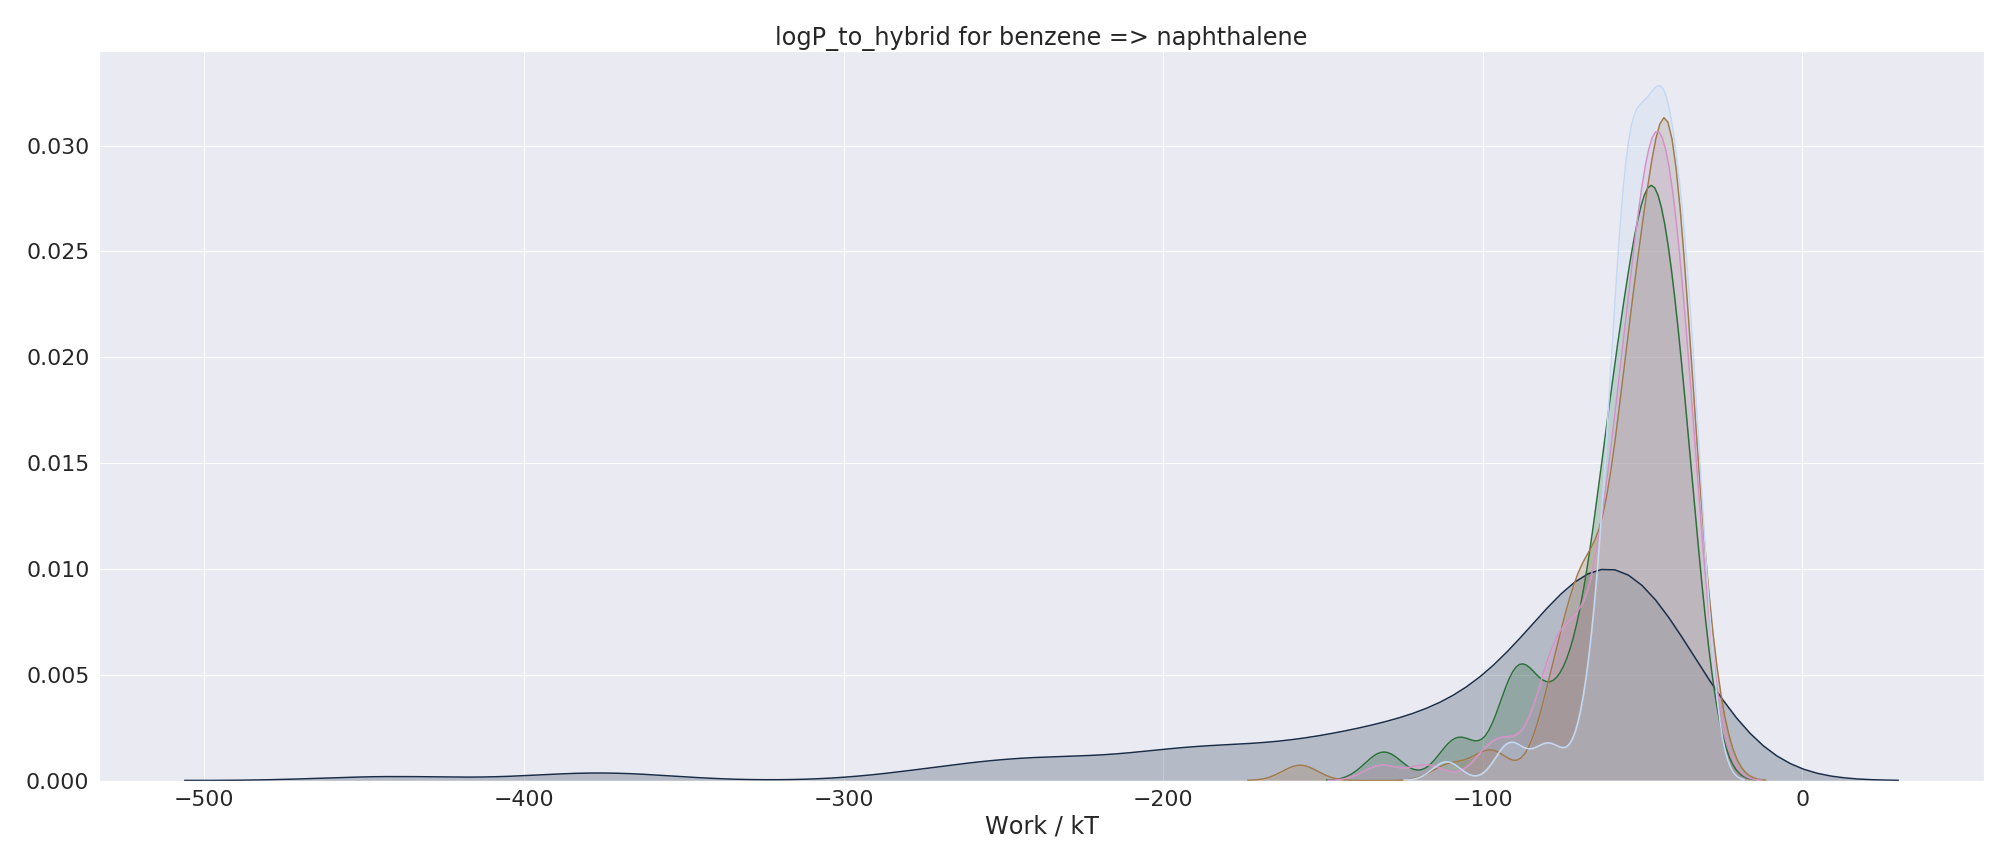
\includegraphics[width=\textwidth]{logP_tohybrid_changebond.png}
    \caption{The distributions of the logP\_to\_hybrid contribution under different initial bond softening parameters. The initial (darkest and broadest) distribution is with no softening; moving to lighter colors, we see the distribution narrow considerably as the initial force constants for bonds connecting unique atoms is scaled by 0.1, 0.01, 0.001, and 0.0001}
    \label{fig:bondsoftening}
\end{figure}
%
In addition to bonds, angles are also represented as harmonic terms, and so it behooves one to examine the effect of softening angles as well, under the same schedule. This time, we will hold the bond softening constant at 1.0 (no softening), and examine the effect of softening the angles in \ref{fig:anglesoftening}
%
\begin{figure}
    \centering
    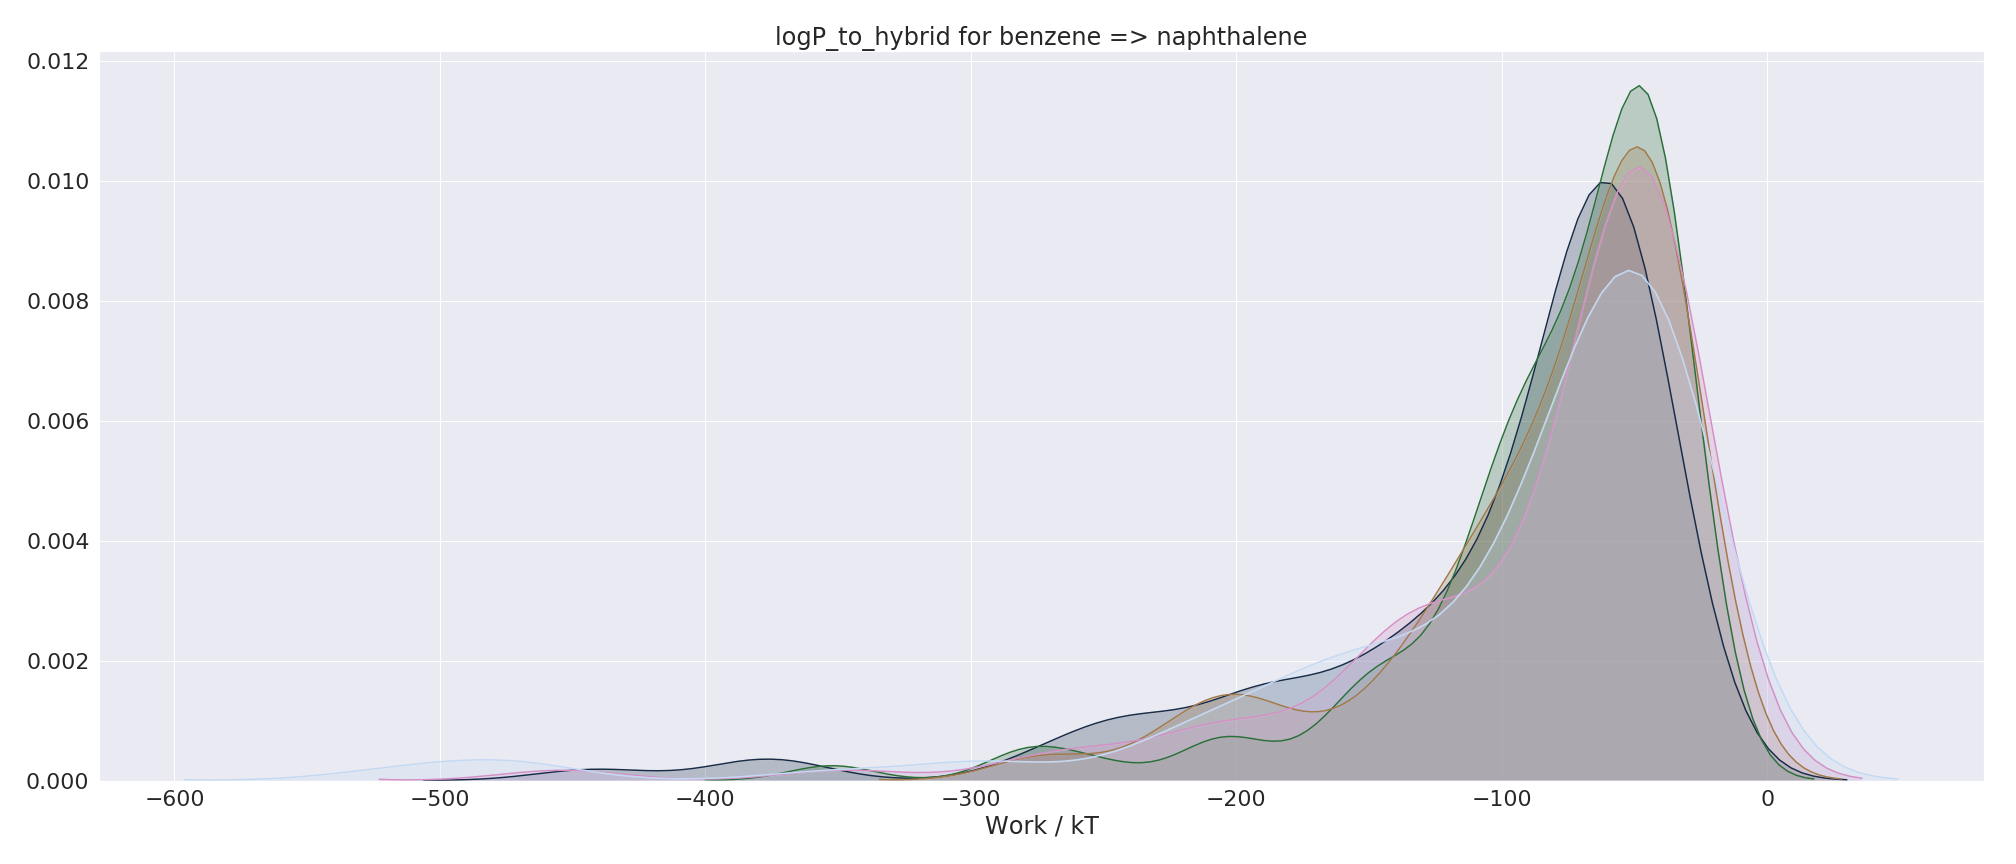
\includegraphics[width=\textwidth]{logP_tohybrid_changeangle.png}
    \caption{The distributions of the logP\_to\_hybrid contribution under different initial angle softening parameters. The initial (darkest and broadest) distribution is with no softening; moving to lighter colors, we do not see the same profound effect as the initial force constants for angles connecting unique atoms is scaled by 0.1, 0.01, 0.001, and 0.0001}
    \label{fig:anglesoftening}
\end{figure}
%
Interestingly, the angle terms do not seem to have the same profound effect as the bond terms.
%
An obvious explanation for this is that the force constants for the angles are considerably smaller, so it may require less softening.
%
In Figure~\ref{fig:softenboth}, I show the same softening schedule for both parameters.
%
\begin{figure}
    \centering
    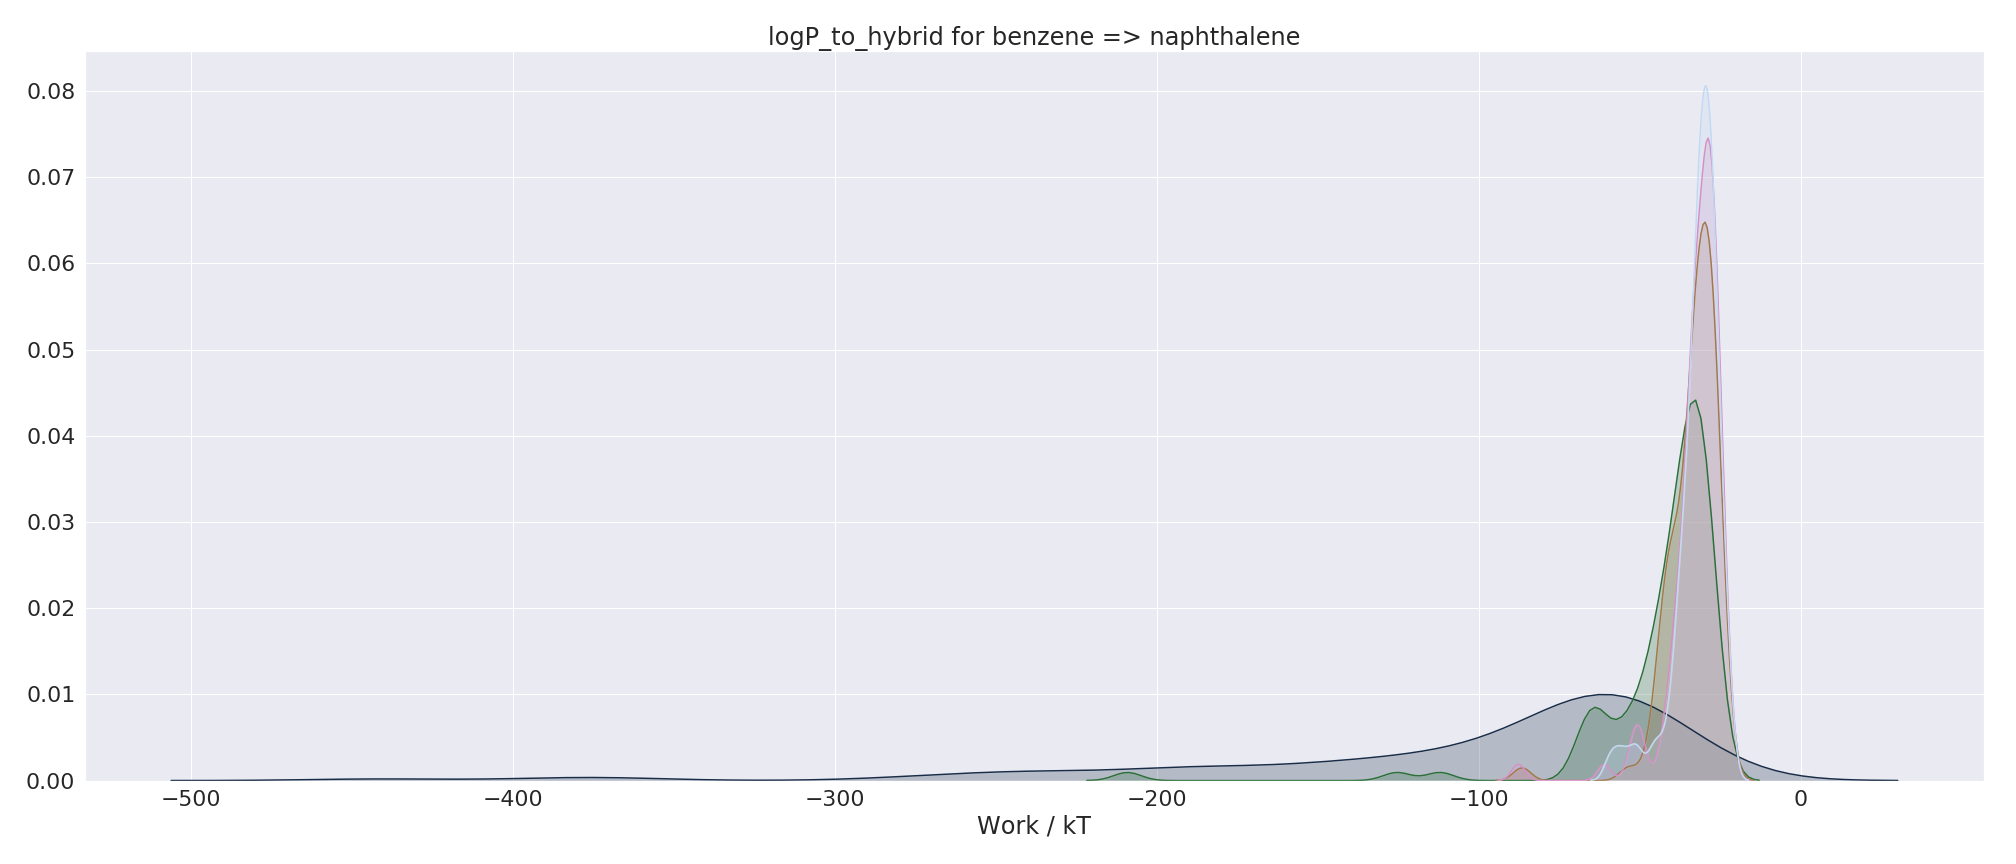
\includegraphics[width=\textwidth]{logP_tohybrid_changeboth.png}
    \caption{The distributions of the logP\_to\_hybrid contribution under different initial angle and bond softening parameters. The initial (darkest and broadest) distribution is with no softening; moving to lighter colors, we see that the distribution grows considerably narrower as both the angle and bond terms are softened to the same degree according to the schedule 0.1, 0.01, 0.001, 0.0001.}
    \label{fig:softenboth}
\end{figure}
%
Taking a closer look at the effect on the standard deviation of logP\_to\_hybrid, Figure~\ref{fig:angle_bond_softening} shows the effect of the different softening parameters on the standard deviation of the logP\_to\_hybrid component. Notably, the angles need not be softened as much as the bonds to reduce the variance of this component. The standard deviation of the standard deviations, obtained by bootstrapping, can be found in Figure~\ref{fig:stdstd}
%
\begin{figure}
    \centering
    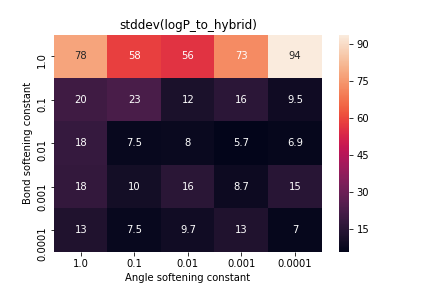
\includegraphics[width=0.8\textwidth]{std_nostd_to_hybrid.png}
    \caption{The standard deviation of the logP\_to\_hybrid component under different combinations of bond and angle softening constants. 
    It is noteworthy that the angles need not be softened nearly as much as the bonds.
    All quantities are in effective units of $k_B T$.
    }
    \label{fig:angle_bond_softening}
\end{figure}
%
\begin{figure}
    \centering
    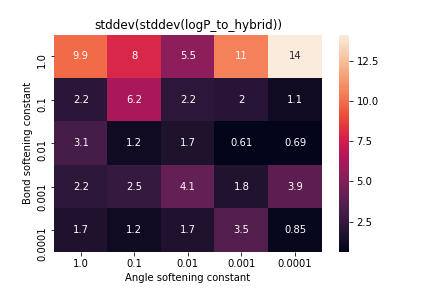
\includegraphics[width=0.8\textwidth]{stddev_lp.png}
    \caption{The standard deviations of the standard deviations of logP\_to\_hybrid under different combinations of bond and angle softening terms.
    All quantities are in effective units of $k_B T$.
    }
    \label{fig:stdstd}
\end{figure}
%
Although we can greatly diminish the variance of this quantity by simply softening the bonds, it is important to keep in mind that the ultimate objective is not to minimize the variance of the jump to the hybrid system, but rather to minimize the variance of the ultimate acceptance probability.
%
It is not difficult to imagine how excessive softening could negatively affect the overall acceptance probability, especially if the dimension matching distribution does not match the softened distribution.
%%
%
\section{Tuning NCMC Protocol length}
%
The simplest hyperparameter to tune in NCMC is the length of the switching protocol. The longer this protocol is, the more favorable the work values.
%
At the same time, the longer protocols require a greater amount of wall clock time.
%
At a certain point, the additional wall clock time consumed by the NCMC simulation is not worth the diminishing benefit in terms of work (which contributes directly to the acceptance probability).
%
Certain transformations may require a longer protocol than others; in this work, I use the same protocol length throughout a calculation.
%
%
\subsection{Limitations of tuning only length}
%
However, tuning the length alone, while straightforward, has limitations.
%
For instance, with a naive protocol linearly switching $\lambda$, it may be necessary to extend the protocol to many steps to ensure reasonable acceptance probabilities.
%
This approach does not give us the opportunity to more freely alter the schedule of the control parameters and potentially gain efficiency.
%
\subsection{Tuning Annealing Schedule}
%
However, with a protocol that may be nonlinear with the control parameter $\lambda$, we may afford ourselves an efficient protocol with many fewer steps.
%
The practical upshot of this is that a shorter protocol can achieve reasonable performance, provided the protocol is reasonable.
%
Unfortunately, as described previously, the thermodynamic length can be relatively difficult to calculate, and will vary depending 
%
\subsubsection{Theory}
%
%
In order to perform the experiment above, I first computed the thermodynamic metric tensor along the one dimensional path.
%
Then, I altered the schedule of control parameters to change $\lambda$ more rapidly when the metric tensor was small (indicating that neighboring distributions are similar) and more slowly when it is large (indicating that neighboring distributions may be quite far apart).
%
Although this sounds like a reasonable task, it is simplified in the case of the harmonic oscillator, where the metric tensor is available analytically.
%
Unfortunately, as is typically the case, the metric tensor is not available analytically for any molecular simulation of interest.
%
Thus, it must be estimated from sampling data, as described in \cite{Minh2011}.
%
This can be a rather expensive process, and may not be worth the added computation time.
%
\subsection{Limitations to tuning annealing schedule}
%
Despite the pleasant straightforwardness of using the metric tensor to define nonequilibrium switching protocols, there is another pitfall besides the computation cost: different pairs of ligands will have different metric tensors for their transformations, as well the same pair of ligands in different environments.
%
This means that it is not straightforward to transfer the values learned from one calculation into another.
%
Coupled with the computational cost, this may make the approach of using the thermodynamic metric tensor infeasible.
%
However, there may be alternate schemes that allow some degree of transfer learning.
%
\subsubsection{Simple solutions}
%
The simplest solution would be to perform a calculation with a number of different ligands in a common environment (such as explicit water) and trying to estimate a metric tensor for each of those transformations.
%
Then, one could potentially utilize a summary statistic of this collection of metric tensors in the hopes that on average, it will perform better than a naive protocol.
%
These approaches need to be explored in greater detail with a large number of different conditions
%
\subsubsection{General Solutions using Machine Learning}
%
In the future, one promising path forward is to use advances in machine learning to predict favorable alchemical paths.
%
In this paradigm, one might take many calculations in different environments, and learn a function $f_{\theta}(\mathcal{M}_1, \mathcal{M}_2)$ with optimizable parameters $\theta$ that maps a pair of molecules $\mathcal{M}_1$ and $\mathcal{M}_2$ to a reasonable schedule of control parameters.
%
Although appealing, it remains to be discovered how such a scheme would account for the myriad environments in which molecules find themselves in the course of a drug discovery program.
%
%
\subsection{Relationship to Geometry Tuning}
%
As mentioned earlier, there exists to some extent a tradeoff between the effort engaged in dimension matching and the effort spent in nonequilibrium switching.
%
More precisely, the more similar the hybrid system at the endpoint is to the non-modified system at the corresponding endpoints, the more straightforward the task of the dimension matching algorithm.
%
However, completely annihilating the valence interactions of newly-added atoms is also potentially dangerous.
%
Atoms that are not anchored to the molecule can easily drift far away, creating additional work as the bonds and angles are scaled on.
%
On the other hand, the dimension matching algorithm can essentially ignore the nonbonded interactions with surrounding atoms, as these are always decoupled at the beginning of the nonequilibrium switching protocol.
%
One question that remains is whether it is worthwhile to include the nonbonded interactions for the sake of maintaining favorable intramolecular nonbonded interactions.
%
%In Figure~\ref{fig:use_nonbonded}, we explore this tradeoff for a simple system of alkanes in vacuum, where %there are no other nonbonded interactions.
%
%\begin{figure}
%    \centering
%    \includegraphics{}
%    \caption{Average acceptance probability across all transitions for different lengths of NCMC with %nonbonded terms enabled in the dimension matching step (blue) and disabled (red).}
%    \label{fig:use_nonbonded}
%\end{figure}
%
\subsubsection{Possibility of resolving poor valence terms}
%
Although initially it seems that softening bonds is deleterious to the acceptance probability, the use of the dimension matching scheme without resampling means that small deviations from the target distribution can easily compound for large proposals.
%
As a result, it seems prudent to offer the choice of softening bonds, angles, and torsions between newly introduced atoms.
%
\nowidow[5]

\chapter{Stochastic Approximation}
%
Having completed the components for preserving the correct equilibrium distribution, I now turn to the task of developing the on-line adaptation scheme for biasing toward states with desirable free energy properties.
%
In order to do this, I turn to stochastic approximation, which has been used successfully in many contexts, especially Monte Carlo~\cite{Robbins1951, Tan2017,Liang2007, Park2006}.
%
\section{Stochastic Approximation for Molecular Simulation}
%
Before deriving the update rule for the present case, I will briefly review applications of stochastic approximation in molecular simulation.
%
Often, when one is simulating from an expanded ensemble, the mixture components (individual discrete states) will have very different free energies.
%
Since the relative population is given by
\begin{equation}
    \frac{p(k=n)}{p(k=m)} = e^{- \beta (\Delta G_n -\Delta G_m)}
\end{equation}
\noindent even small differences in free energies will result in very large differences in relative populations.
%
Practically speaking, this results in only rarely calculating acceptance probabilities between certain states, and therefore poor statistics in the final estimate of relative free energies.
%
To resolve this, one approach is to attempt to flatten the histogram of states.
%
In order to achieve this flattening, one could use the expanded ensemble weights $g_k$ add additional weight to those states with a lower free energy.
%
This requires knowing the relative free energies, however, defeating the purpose of running the algorithm in the first place.
%
Therefore, many adaptive schemes have been developed to estimate these weights online, such as in \cite{Wang2001} \cite{Tan2017} \cite{Liang2007}.
%
\subsection{SAMS}
%
Recently, a formulation of stochastic approximation Monte Carlo was developed by Tan \cite{Tan2017} that is asymptotically optimal in the sense of minimizing the variance of the weights $g_k$.
%
This algorithm is performed as follows:
%
\begin{eqnarray} \label{binary-sams-sa}
     g^{(t-1/2)}_k = g^{(t-1)}_k - t^{-1} \frac{\delta_{s_t,k}}{\pi_k} \\
     g^{(t)}_k = g^{(t-1/2)} - g^{(t-1/2)}_1
\end{eqnarray}
%
\noindent where each $g^{(t)}_k$ is the adapted weight of chemical state $k$ at iteration $t$, $s_t$ is the current state at iteration $t$, and $\pi_k$ is the target probability for state $k$.
%
Setting each $\pi_k = \frac{1}{n}$ for a system with $n$ states will result in even sampling, and asymptotically will result in weights equal to the relative free energies \cite{Tan2017}.
%
%
Its simplicity, combined with its asymptotic optimality~\cite{Tan2017}, makes it an appealing choice for adaptively reweighting the components of the expanded ensemble.
%
Although this can be very useful for determining the entire set of pairwise relative free energies, it can still be very burdensome for large sets of chemical states.
%
In general, we are not interested in merely even sampling, as we are not concerned with the relative free energies of two unfavorable chemical states.
%
Therefore, we seek an adaptive algorithm that provides for greater sampling of chemical states that are favorable according to some free energy criterion.
%
\section{Doubly-recursive SAMS}
%
In general, in physical simulation tasks, we seek states that optimize a free energy difference between multiple states, not simply a single state.
%
For instance, if we are optimizing to maximize binding affinity, the quantity we seek to maximize is (omitting constants) the association constant $K_a$:
%
\begin{equation}
    K_a \propto \frac{Z_{PL}}{Z_{P}Z_{L}}
\end{equation}
%
\noindent where $Z_*$ represents the normalizing constant of the appropriate species $*$, $P$ and $L$ represent protein in solvent and ligand in solvent systems respectively, and $PL$ represents the interacting protein-ligand complex system.
%
Since we are trying to find the chemical state which maximizes this quantity, we are generally interested in so-called relative free energies.
%
As a result, when comparing two ligands, $L_1$ and $L_2$, we have:
\begin{eqnarray}
     K_{a,1} &=& \frac{Z_{PL_1}}{Z_{P}Z_{L_1}} \\
     K_{a,2} &=& \frac{Z_{PL_2}}{Z_{P}Z_{L_2}} \\
     K_{relative} &=& \frac{K_{a,1}}{K_{a,2}} = \frac{\frac{Z_{PL_1}}{Z_{P}Z_{L_1}}}{\frac{Z_{PL_2}}{Z_{P}Z_{L_2}}} = \frac{\frac{Z_{PL_1}}{Z_{L_1}}}{\frac{Z_{PL_2}}{Z_{L_2}}} = \frac{Z_{PL_1}}{Z_{PL_2}} \frac{Z_{L_2}}{Z_{L_1}}
\end{eqnarray}
%
\noindent Therefore, if we would like a chemical state to be sampled according to its relative binding affinity, we need to adapt the weights of the chemical states such that
%
\begin{equation}
    p(k) \propto \frac{Z_{PL_k}}{Z_{L_k}}
\end{equation}
%
That is, the target weights $\pi$ must be adapted as well, since we do not know \emph{a priori} what the relative free energies are.
%
\subsection{Description of Algorithm}
%
More generally, consider we have $s$ different probability densities:
%
\begin{eqnarray}
p_{ij}(x) &=& e^{g_{ij}^*} q_{ij}(x) \:\:,\:\: i = 1,\ldots, s\:\:, \:\: j = 1,\ldots, m
\end{eqnarray}
%
and we desire to design a chain where the marginal distributions of all $s$ chains are
%
\begin{eqnarray}
p_{ij} &\propto& \prod_{i'=1}^s e^{-\theta_s g_{i'j}^*} = \exp\left[ - \sum_{i'=1}^s \theta_s g_{i'j}^* \right] \forall i = 1,\ldots, s
\end{eqnarray}
%
where the \emph{design vector} $\Theta \equiv \{ \theta_1, \ldots, \theta_s \}$ specifies how different targets and antitargets are used in weighting the design constraints.
%
We postulate that we can do this by defining $\pi_i(Z)$ for $Z \equiv \{g_1, \ldots, g_s\}$ as
%
\begin{eqnarray}
p_{ij}(Z | \Theta) &\propto& \exp\left[ - \sum_{i'=1}^s \theta_s g_{i'j} \right]
\end{eqnarray}
%
\section{Toy Examples}
%
Having described the algorithm in principle, I now present a simple toy example to empirically see that the quantity of interest is generated.
%
In this example, we simulate a set of harmonic oscillators:
\begin{eqnarray}
    p_{i0} \propto e^{-\beta \frac{K_{i0}}{2} (x - x_{i0})^2} \\
    p_{i1} \propto e^{-\beta \frac{K_{i1}}{2} (x - x_{i1})^2}
\end{eqnarray}
%
As a model of the binding free energy calculation, we would like:
\begin{equation}
    p_{1}(k) \propto \frac{Z_{1_k}}{Z_{2_k}}
\end{equation}
%
\noindent where the subscripts 1 and 2 indicate the different chains (analogous to complex and solvent for the binding free energy).
%
\begin{figure}
    \centering
    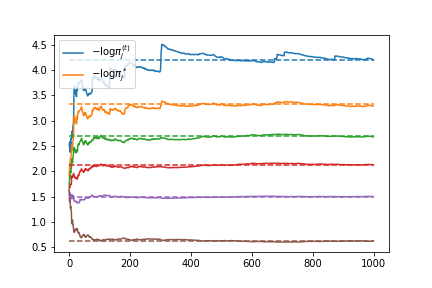
\includegraphics{logpitrace_s_nosep.png}
    \caption{The target weights of the various harmonic oscillators (solid) and the true value (dotted line). Note that the higher free energy states take significantly longer to converge to their true values}
    \label{fig:toy_doublesams}
\end{figure}
%
As can be seen in Figure~\ref{fig:toy_doublesams}, the target weights of the favorable states (lower free energy) converge faster.
%
This is what we desire, since we are not interested in how much more unfavorable one high free energy state is from another.
%
We can extend this principle to multiple chains as well; as generalized above, this applies to cases such as multitargeting (finding chemical states with a favorable free energy in multiple chains) or selectivity (finding states that are favorable for one but not another). 
%
\subsection{Performance}
%
Ultimately, the goal of the algorithm is to more quickly explore relevant regions of chemical space.
%
However, there are some limitations to the stochastic approximation algorithm presented here that are worth discussion.
%
\section{Limitations}
%
Two issues arise when discussing the limitations of the stochastic approximation algorithm used here.
%
The first is the convergence rate. Since the algorithm works by counting the numbr of times different states are visited, it can take a lengthy simulation before the chemical state space begins to be explored.
%
The second limitation is that the SA algorithm presented here is designed for a fixed number of states.
%
However, it is clear that to truly carry out molecular design, an algorithm must be capable of handling the situation where the number of states is not known \emph{a priori}.
%
This can arise, for instance, when the proposal distribution is a neural network.
%
\subsection{Convergence Rate}
%
The first topic of concern is the convergence rate.
%
To examine this in greater detail, we observe behavior in a toy model.
%
Even in the traditional binary SAMS update (described in \cite{Tan2017}), it can take many iterations to begin to achieve even sampling, especially if the mixture components are kinetically separated.
%
\begin{figure}
    \centering
    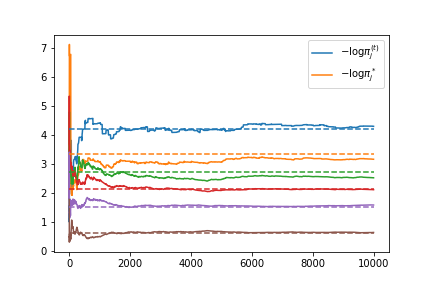
\includegraphics{logpitrace_s_smallsep.png}
    \caption{Convergence of binary SAMS from a single realization of harmonic oscillators with only a small separation in means.}
    \label{fig:smallsep}
\end{figure}
%
In Figure~\ref{fig:smallsep}, one can see that the desired target weights (dotted lines) are quickly approached by the adapted target weights (solid lines), and are more quickly approached for low free energy states than others.
%
However, what happens if we add a small amount of kinetic separation to these harmonic oscillators?
%
In principle, this issue is resolve by nonequilibrium switching; however, in practice, efficiently resolving these types of issues is quite difficult, especially when the states between which one must transition are so diverse.
%
More work needs to be performed to not only initialize the weights well, but investigate the possibility of initial algorithms that may approach the desired target more quickly than the asymptotic algorithm.
%
\subsection{Number of States}
%
Ideally, we'd be able to jump to new (unseen) chemical states, which would enable molecular design in a truer sense.
%
However, the formulation of the SA algorithm above clearly is designed for a fixed number of states.
%
One way to resolve this is to imagine that, although more states may be added on the fly, we set an upper limit on how many states can be explored.
%
In this case, we will eventually reach the maximum number of states, at which point the algorithm obviously becomes the double recursion SA above.
%
However, there are some questions regarding this.
%
We already saw that the convergence of the algorithm is highly sensitive to the mixing of the underlying sampler; what happens when the number of states changes?
%
This is a subject that calls for further investigation and future work.
%
\section{Weight initialization}
%
One major challenge with SAMS algorithms is how the weights are initialized.
%
The initial weights will have a profound effect on the performance, especially as weight adaptation diminishes.
%
For this reason, many use a multiple-stage scheme as in \cite{Tan2017}; this allows the weights to initially adapt much more quickly, and then revert to the asymptotically optimal gain decay after a certain condition is reached.
%
In addition to this scheme, it is advantageous to determine whether there exists simple tricks that can initialize the SAMS weights nearer the correct target than zero.
%
\subsection{Implicit volume term}
%
One issue that the reversible jump-based simulation incurs that most others do not is that the dimensionality of phase space changes with the chemical state.
%
As a result, depending on the units used, there is a volume term that is not accounted for in the acceptance probability.
%
Since in free energy calculations we are always looking at differences, this is not a concern for accuracy, but is for efficiency, since this term will cause certain states to become very unfavorable based on the number of degrees of freedom in that state.
%
Observing this discrepancy, I decided to initialize the stochastic approximation weights for each state using a very rough guess of the implicit volume term: 
%
\begin{eqnarray}
g_k^0 &=& n_{heavy}*4.5 + n_{hydrogen}*3.8
\end{eqnarray}
%
The hydrogen term is smaller because it only has two degrees of freedom (bonds are constrained).
%
\subsection{Hydration}
%
A common environment in relative free energy calculations is the solvent phase, which consists of just the small molecules in solvent.
%
Since the environment is essentially the same in solvent regardless of the target, it is advantageous to develop a quick initialization scheme that can be easily reused.
%
Here, I implemented one scheme, however, there exists the potential for other schemes to be developed as well.
%
\subsubsection{Initialize with minimized point energies}
%
One interesting approach for initializing weights in the solvent phase is to use the minimized point energies of the corresponding molecule in implicit solvent.
%
In \cite{mobley2008} this approach was explored as an approximation to the hydration free energy of the molecule.
%
Since we do not rely on the initialization of weights for correctness, only for efficiency, a simple scheme like this one is useful.
%
It is possible that more sophisticated implicit solvent models (such as PBSA~\cite{Tan2006}) would produce superior starting weights, but the added cost may not be justified.
%
%
\subsection{Complex weight initialization}
%
In molecular design problems relating to drug discovery, another common phase is the complex phase--that is, protein and ligand interacting in solvent.
%
This phase usually contains systems that have many more atoms, as well as much longer correlation times.
%
Therefore, it would be extremely helpful to have an efficient weight initialization scheme.
%
However, the complex phase poses several additional challenges.
%
One challenge is that the relative free energies of different chemical states in the complex phase cannot be as easily estimated as in the solvent phase.
%
Another is that the complex phase varies greatly between different projects; one cannot come up with a single, simple initialization scheme for all complex phase calculations as one can for the solvent phase.
%
However, there are several ideas that may be implemented.
%
%
\subsubsection{Initial acceptance probability}
%
One simple idea is to use the initial $\ln P_\mathrm{accept}$ values that are generated by the algorithm.
%
This is appealing intuitively, because $P_\mathrm{accept}$ is a (very poor) estimate of the relative free energy of the two states~\cite{Zwanzig1954}, as well as being produced as a byproduct of the algorithm (requiring no additional effort).
%
However, there are several pitfalls to this approach. 
%
In particular, due to the potentially high variance of the $P_\mathrm{accept}$, setting a stochastic approximation weight with it can result in an initialization extremely far from the true value.
%
This would actually make the simulation even less efficient.
%
One approach would be to only initialize the weight with the initial acceptance probability if the log acceptance probability is within some bounds.
%
This might prevent the SAMS weights from being initialized to quantities very far from the true value, while still allowing a decent initial guess.
%
%
\subsubsection{Machine learning score}
%
Another approach not explored here would involve using a machine learning algorithm that attempts to predict binding free energies~\cite{Colwell2018, Wu2018} to initialize the weights.
%
A caveat here would be that a machine learning algorithm that is more accurate or otherwise has a different error pattern than the forcefield might start the weights farther from the desired true values (even if they are more accurate in reality).
%
The area of weight initialization represents a fertile ground for future investigation.
%
\subsubsection{Implicit ligand theory}
%
Another interesting area of research is implicit ligand theory~\cite{Nguyen2018,Xie2017,Minh2012impl, Minharxiv}, which uses one or more snapshots of a rigid protein and simulates only the small molecule, resulting in an impressive speedup.
%
These rapidly-calculated approximations could be used to initialize the weights, providing a potentially profitable starting point.

\chapter{Alternative to SA: Highly Parallel Nonequilibrium Switching}

\section{Introduction}
%
As discussed, there are several limitations of the stochastic approximation (SA) algorithm.
%
However, that does not preclude the use of the reversible-jump (RJ) algorithm in other clever ways.
%
For a long time, it has been known that rather than accepting or rejecting a proposal attempt, one can cache the resulting acceptance probability and use it to estimate the free energy difference offline.
%
In molecular simulation, this technique is known as nonequilibrium switching~\cite{Hummer2001, Aldeghi2018}, and in statistics as annealed importance sampling (AIS)~\cite{Neal2001}.
%
Examples of estimation techniques include the exponential averaging estimator~\cite{Zwanzig1954}, as well as the optimal Bennett Acceptance Ratio (BAR)~\cite{Bennett1976,Shirts2005,Crooks1999Thesis, Meng1996}, which uses bidirectional data.
%
Though this has not often been utilized for free energy calculations, it has several appealing advantages in the modern age.
%
First, it is highly parallelizable--unlike SAMS-like expanded ensemble algorithm, it can easily run many switching trajectories or proposal attempts simultaneously.
%
With hardware becoming increasingly parallel and the availability of cloud computing, this is an attractive feature.
%
Second, there is no need to wait for a sampler to explore all the states--by definition of the algorithm, the user can choose which states.
%
Third, it is still possible to employ a wide range of adaptive algorithms.
%
For instance, one could use Bayesian experimental design~\cite{Vanlier2012, DasGupta1996} to iteratively choose how to allocate effort to different "legs" of the calculation.
%
\section{Advantage of RJ Nonequilibrium Switching}
%
Since codes for nonequilibrium switching based relative free energy calculations already exist, one might wonder what advantage the complication of reversible jump brings.
%
In order to understand why one would undertake this approach, consider what is required for a standard nonequilibrium switching based relative free energy calculation.
%
In Figure~\ref{fig:trad_neq}, one can see that the typical setup of a nonequilibrium free energy calculation is to run simulations at the alchemical endpoints (that is, a hybrid system with the control parameters set to either 1.0 or 0.0), and periodically generate proposal attempts to reach the other endpoint.
%
This requires simulation of the hybrid system at both endpoints for each pair for which one would like to calculate the free energy difference.
%
Note that in this scheme, one cannot use the equilibrium simulation used in a calculation for $\Delta\Delta_{AB}$ to, for instance, estimate $\Delta\Delta_{AC}$, where $A,B,C$ are molecule indices.
%
This is because the alchemical system must contain all the degrees of freedom of both endpoints, which will not necessarily include the degrees of freedom of the rest.
%
\begin{figure}
    \centering
    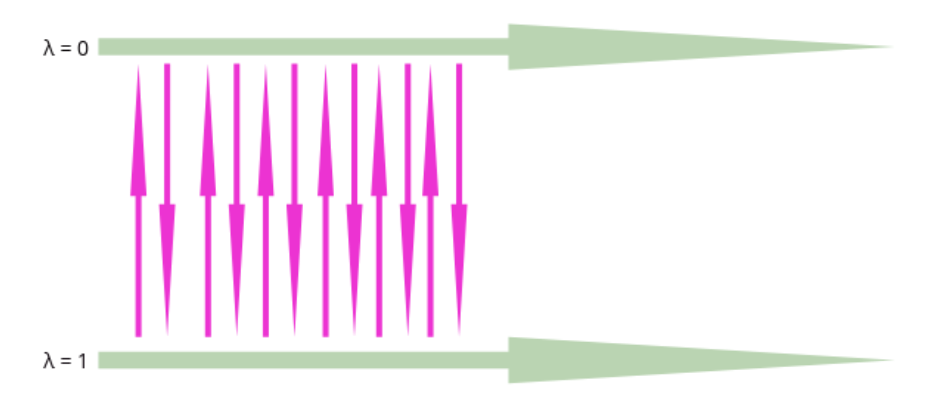
\includegraphics[width=1.0\textwidth]{new_neqdiagram.png}
    \caption{Illustration of a nonequilibrium switching free energy calculation. Note the requirement for simulation at the alchemical endpoints. The horizontal green lines represent the equilibrium simulations at each endpoint, while the magenta lines depict the switching trajectories from samples of each state to the other.}
    \label{fig:trad_neq}
\end{figure}
%
However, using the reversible jump scheme, one simulates from the \emph{nonalchemical} endpoints for each molecule, and then in the course of the nonequilibrium switching trajectory, inserts the missing degrees of freedom and removes the superfluous degrees of freedom.
%
This means that, to use the previous abstract example, one can simply run multiple equilibrium simulations, then adaptively choose which pairs should be emphasized.
%
It would also allow new molecules to be added without re-simulating any of the existing molecules in the set; in principle, if one wanted a fast estimate, the exponential averaging estimator could even be used to without performing any additional equilibrium simulation.
%
Additionally, the reversible jump scheme enables ring formation and breakage without resorting to more sophisticated tricks, which allows a much greater freedom for the user to choose different 
%
Finally, an adaptive design scheme based on Bayesian experimental design could easily incorporate other non-free-energy-based objectives, such as a model of synthetic accessibility or some other desirability criterion.
%
\section{Use of cloud computing resources}
%
This approach to the reversible-jump based algorithm presented in this thesis opens the door to ready use of cloud resources such as Amazon Web Services, which are already being employed in free energy simulations~\cite{Cournia2017}.
%
Offerings such as AWS not only enable users without in-house clusters to use high-performance hardware, but also enhance the reproducibility of research.
%
Entire stacks used to perform computation can be exported via services such as AWS CloudFormation, enabling rapid and straightforward reproduction of research.
%
Another benefit of using on-demand cloud resources is that it enables the direct application of economics to the question of calculation efficiency.
%
Rather than comparing algorithms in terms of asymptotic variance or other similar criteria, we can now compare them in terms of their dollar cost; how much do we have to spend in order to achieve the desirable result?
%
This also allows us to put a direct price tag on speed improvements.
%
While questions such as the variance of the acceptance probability once seemed abstract, they now strike our wallets.
%
Since we are performing calculations on groups of molecules, we can also use this cost data to determine which edges are most profitable to explore, and which can be estimated by summing other edges.
%
As in \cite{Wang2015}, the presence of cycles could also be used to correct for errors in the calculation.
%
\section{Pricing and Economics of Cloud Computing}
%
Due to familiarity, the remainder of this chapter will use Amazon Web Services as an example.
%
Using AWS for molecular simulation, there are several cost considerations:
\begin{itemize}
    \item Storage of input and output
    \item Compute time
    \item Data egress (ingress is free)
\end{itemize}
%
Here, I will primarily discuss the issue of compute time.
%
There are several pricing models on AWS and its competitors for compute time.
%
On-demand pricing refers to the use of resource at a fixed hourly price.
%
So-called spot pricing allows users to bid on unused capacity at a significantly reduced price.
%
This price fluctuates, however, and is not guaranteed to remain under the user's bid.
%
In the present situation, this is tolerable: if an instance is killed because it becomes prohibitively expensive, we lose whatever nonequilibrium switching it has performed but not copied to storage, but nothing else.
%
At the time of this writing and in the geographically nearest datacenter, the price of a single GPU instance hovered near \$0.27 per hour.
%
In preliminary investigations on a GTX-Titan, a full proposal of 10ps from one alkane to another takes approximately 60 seconds.
%
In other words, we can compute over 100 switching attempts for just 50 cents!
%
Of course, this is a small system--scaling up will be pricier. 
%
These price signals can also guide the investigator into the most effective use of his or her time and money.
%
However, this illustrates the low cost of the algorithm on modern infrastructure, and also highlights that pairs of molecules for which is advantageous to compute many switching attempts can be done cheaply and in parallel.
%
One may be left wondering why one couldn't simply use many replicates of the stochastic approximation algorithm to take advantage of the parallelism.
%
One could do this, of course, and whether this is efficient in terms of processor or wall clock time requires empirical investigation.
%
However, one feature of the low spot pricing is its volatility--a user cannot rely on the price remaining at its current level indefinitely.
%
In fact, this aspect has motivated interesting research in modeling the price of spot resources~\cite{Javadi2011} that can be brought to bear on this application.
%
Since the nonequilibrium switching trajectories are independent of each other, loss of some compute resources is not devastating.
%
If necessary, the number of nonequilibrium switching trajectories being performed in parallel can be reduced to save money when the cost increases.
%
Effort can be adaptively reallocated by whatever model or heuristic the user desires.
%
However, if one suspends a chain exploring chemical space due to cost, one loses the adaptation that that chain has already performed.
%
There may exist powerful methods of coupling the stochastic approximation weights, but this is a topic for future research.
%
\subsection{Factors affecting performance}
%
One factor affecting performance is the nonequilibrium protocol itself. 
%
Another factor that could potentially affect performance of this algorithm is the correlation time of the equilibrium simulation.
%
Unlike the SAMS case, where the algorithm accepts or rejects moves to different chemical states, this approach does not benefit from the potential decorrelating effect of changing chemical states.
%
Additionally, the number of parallel computing devices available will profoundly affect whether this choice is a feasible one.
%
With a large number of processing devices, this approach can reduce wall clock time, but empirical evaluation is necessary to determine whether for relative free energy calculations this approach is comparable in efficiency to equilibrium staging.

\chapter{Hydration free energy}

\section{Introduction}
%
In this example, we seek to compute the relative hydration free energies of different ligands in explicit solvent.
%
We will use the approach of transdimensional nonequilibrium switching to compute relative hydration free energies for a set of molecules in the FreeSolv dataset~\cite{Mobley2014,DuarteRamosMatos2017}, a set of experimentally and computationally characterized hydration free energies for small molecules.
%
Although this is a simple test, it demonstrates that the algorithm is capable of efficiently producing low-variance work values in explicit solvent, and among diverse sets of ligands.
%
For the example presented in this chapter, we will be using a randomly selected subset of substituted benzene molecules.
%
For each pair of ligands, we will run 1 nanosecond of equilibrium simulation and a nonequilibrium switching protocol 5 picoseconds long. 
%
We will use 1000 switching trajectories in the forward and reverse direction for each pair, and then use the work values to estimate the relative free energies.
%
\section{Thermodynamic Cycle}
%
In order to compute the relative hydration free energy, we employ a thermodynamic cycle wherein we transform the small molecule from one molecule to another in solvent and in vacuum, and subtract the resulting free energies, depicted in \ref{fig:thermocycle}.
%
\begin{figure}
    \centering
    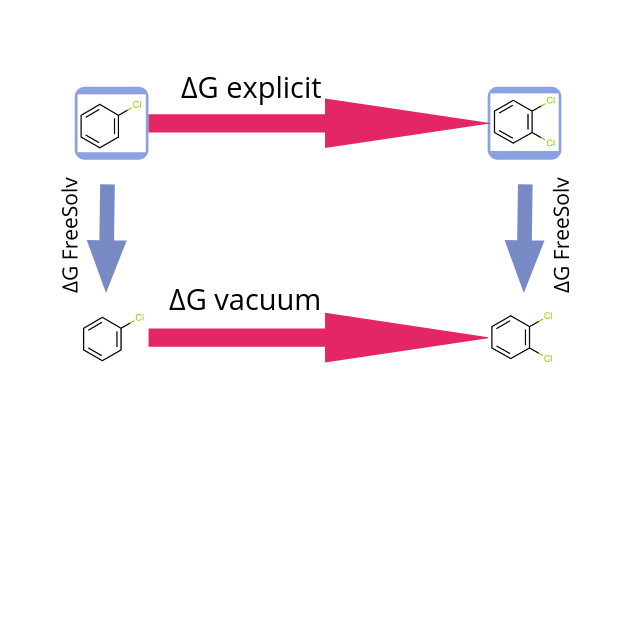
\includegraphics[width=1.0\textwidth]{thermocycle.png}
    \caption{The thermodynamic cycle of the hydration free energy calculation. Blue arrows denote the data available in FreeSolv; magenta arrows denote the legs performed in this work.}
    \label{fig:thermocycle}
\end{figure}
%
We compare to FreeSolv~\cite{Mobley2014}, which is a database of computed absolute hydration free energies; therefore, in order to compare our results to FreeSolv, we will need to compute relative hydration free energies from the absolute data.
%
\section{Vacuum Phase}
%
For the vacuum phase of the simulation, we performed 1 ns of equilibrium simulation for each molecule, and 100 switches between each pair in both directions.
%
For the nonequilibrium switching length, we used 5ps, as it was sufficient for explicit solvent, and so should be sufficient for vacuum.
%
%
\subsection{Explicit Phase}
%
\subsection{Nonequilibrium switching protocol length}
%
Prior to performing this calculation, we performed a quick check of the performance of various nonequilibrium switching times vs. the amount of work that was performed.
%
In this check, we simulated benzene and naphthalene in solvent for 1 nanonsecond, and then performed 100 switching trajectories in each direction.
%
We collected the data and analyzed the standard deviation of the work performed by the protocol, shown in Figure~\ref{fig:benz_naph_protocol_work}
%
\begin{figure}
    \centering
    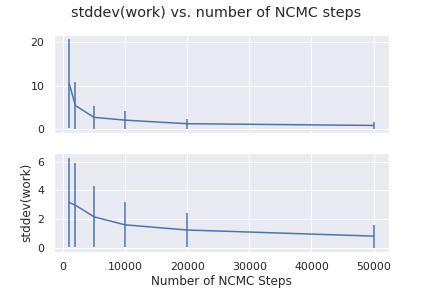
\includegraphics[width=1.0\textwidth]{benz_naph_work_vs_steps.png}
    \caption{The standard deviation of the work for an NCMC switching trajectory between benzene and naphthalene vs. number of steps, with a 1fs timestep. Top: work for transforming benzene into naphthalene. Bottom: work for transforming naphthalene into benzene.}
    \label{fig:benz_naph_protocol_work}
\end{figure}
%
Given that the transformation from benzene to naphthalene is rather difficult without extra bond and angle softening, we decided to use a switching time of 5~picoseconds, and 1000 switching attempts between each pair in each direction.
%
\section{Analysis of the work of the entire move}
%
In addition to the protocol work, we can also examine the distributions of the work of the entire move in both directions.
%
Since this is the quantity that is fed into BAR, it is critical to examine.
%
In \ref{fig:worka}, there is a representative pair of work distributions.
%
\begin{figure}
    \centering
    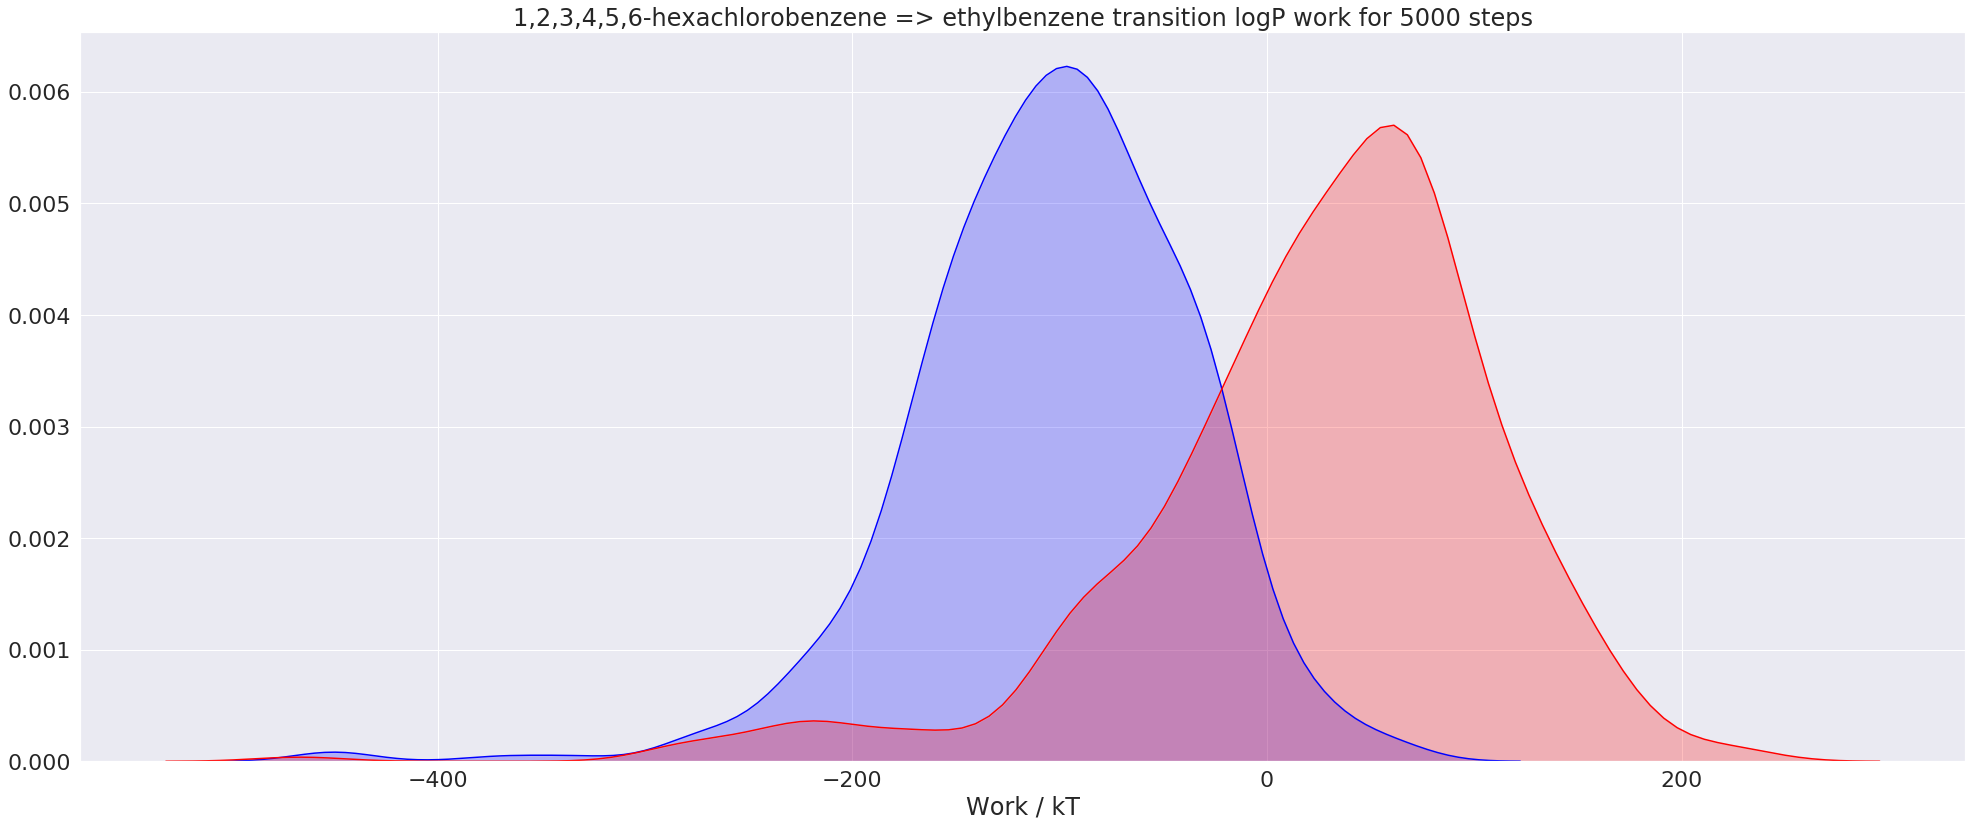
\includegraphics[width=1.0\textwidth]{hexachlor-ethylbenz.png}
    \caption{The forward and reverse (blue and red, respectively) log acceptance probability distributions for transitions between hexachlorobenzene and ethylbenzene. Although the variances of the distributions appear high, the overlap is very good, allowing a low-error free energy estimate.}
    \label{fig:worka}
\end{figure}
%
%
Once again, there appears to be sufficient overlap for proceeding with the estimation of free energy differences.
%
Surprisingly, even in \ref{fig:workb}, the overlap is quite good.
%
\begin{figure}
    \centering
    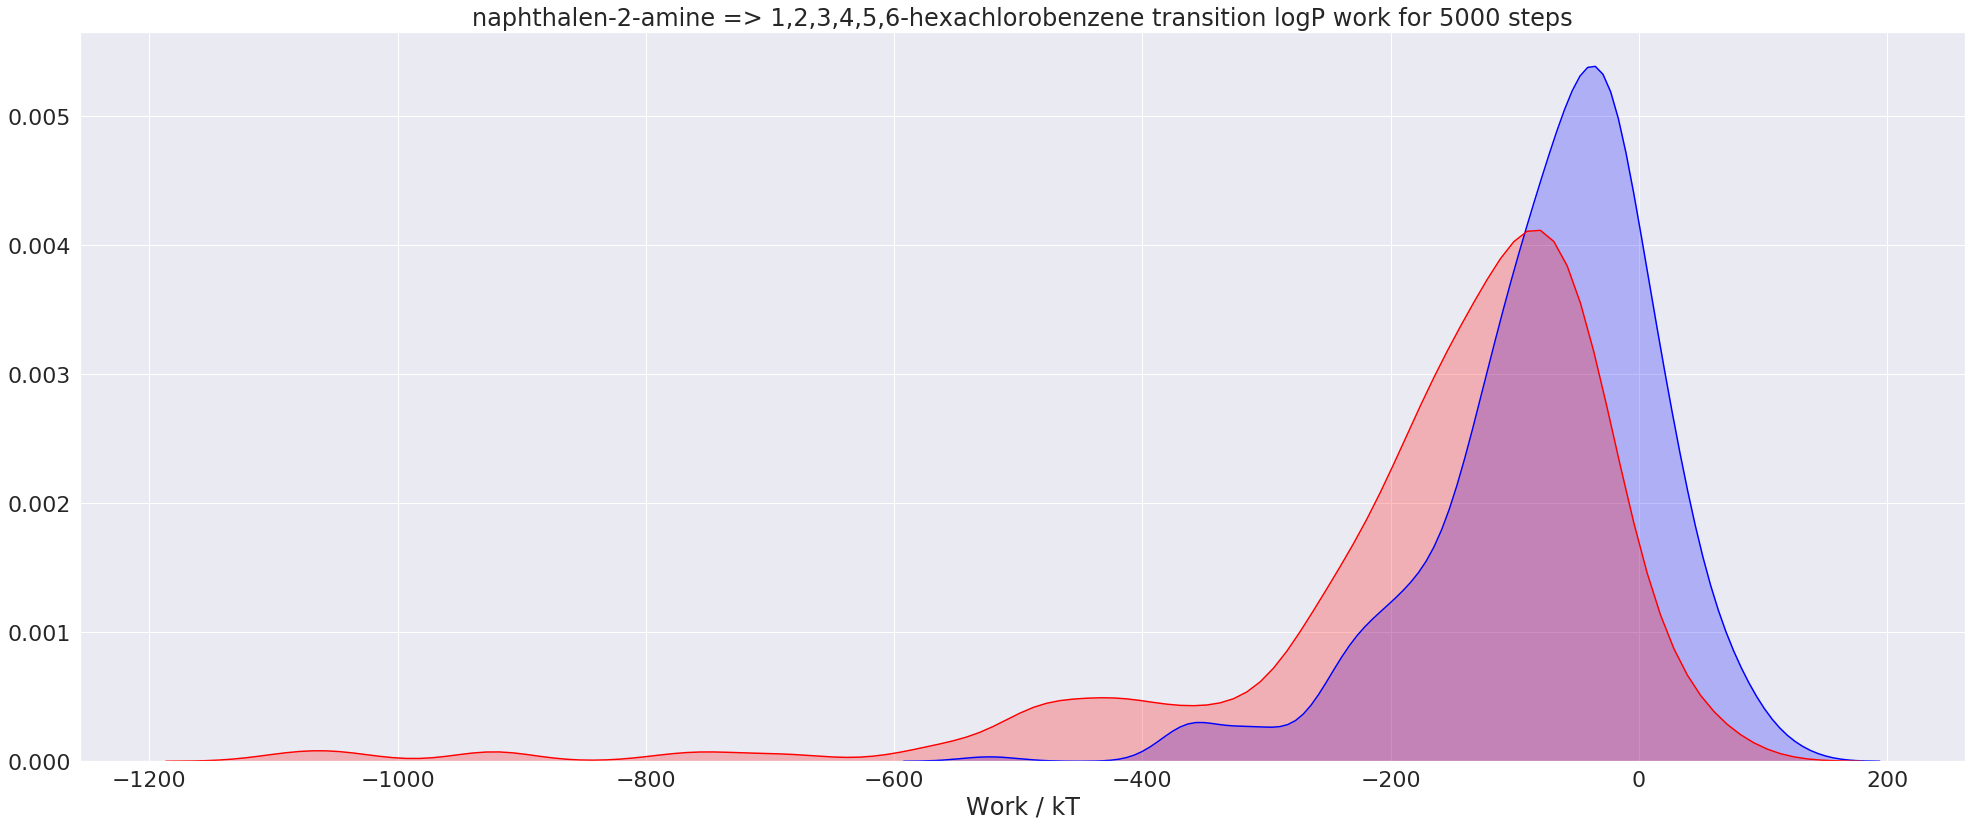
\includegraphics[width=1.0\textwidth]{napthamine-hexachlor.png}
    \caption{The forward and reverse (blue and red, respectively) log acceptance probability distributions for transformations between napthalene-2-amine and hexachlorobenzene. Despite having to create or break a fused ring, the overlap is still quite good, allowing low variance free energy estimates}
    \label{fig:workb}
\end{figure}
%


\chapter{Conclusion}
%
\section{Contributions of work}
%
This work makes several novel contributions to the field.
%
First, this work develops a theoretically rigorous algorithm for simulations that can explore multiple chemical states in a single simulation.
%
This relieves the restriction that most free energy calculation methods have, which is that they only compute relative free energy differences between one pair of ligands, or, in certain cases, a small set.
%
Second, this work provides a theoretically rigorous approach to the formation of ring formation and breaking.
%
Finally, the algorithm presented herein allows for adaptive approaches that have heretofore been impossible.
%
\section{Exploration of Chemical Space}
%
The first goal that this work accomplished was the introduction of a formal and rigorous basis for approaches such as Chemical Monte Carlo (CMC)~\cite{Pitera1998}.
%
While the concept of CMC is attractive, there was no basis to guarantee that the sampling algorithm would be asymptotically correct.
%
By resorting to Reversible Jump MCMC~\cite{GREEN1995}, I am able to provide a basis for jumps in chemical space that provably preserves the correct invariant distribution, allowing the application of additional techniques such as stochastic approximation.
%
\subsection{Chemical State Proposals}
%
The first part of the work addresses the requirements as well as the possibilities for making proposals to jump to different chemical states.
%
Unlike in previous algorithms such as Multisite Lambda Dynamics~\cite{Knight2011}, the set of ligands that one chooses for a calculation can be quite diverse.
%
As such, a mechanism of efficiently proposing jumps from one state to another must be developed.
%
In addition to setting forth the conditions for correctness, one must also develop a method that is reasonably efficient.
%
Although formal statements exist to define which chemical states would be most "near" each other in a sense, known as thermodynamic length~\cite{Crooks2007}, these expressions are intractable to compute.
%
Therefore, one must resort to heuristics.
%
As a first attempt, I used the number of atoms deemed to be in common between the current and proposed molecule by a maximum common substructure search (MCSS), itself an algorithm with several hyperparameters.
%
I conducted an exploration of various parameters for the MCS search, determining that for some pairs this is a highly influential setting, while for others it matters far less.
%
Finally, I presented groundwork for future work in the realm of chemical state proposals, especially techniques that would allow for a chemical space that is not predefined in the beginning of the calculation.
%
I also described aspects of the algorithm that can be combined with the power of machine learning to leverage the best of both techniques.
%
\subsection{Dimension Matching}
%
Once it is decided to attempt a jump to a new chemical state, with atoms assigned to one molecule, the other, or both, the task becomes to insert the missing atoms and delete the ones that do not belong to the following state.
%
This procedure, known as dimension matching, is a critical component of the algorithm.
%
First of all, there are several important requirements that must be imposed.
%
The proposal must be accompanied by a normalized proposal probability to compute the requisite acceptance test.
%
Second, the proposal must be exact--that is, it cannot be drawn by an approximate scheme (such as most MCMC algorithms).
%
Third, the probability of proposing atoms that are being deleted must also be computable exactly.
%
These restrictions combine to eliminate several straightforward approaches to inserting missing atoms.
%
In this work, I developed a scheme based on Configurational Bias Monte Carlo (CBMC)~\cite{Siepmann1992} that meets all of these criteria.
%
This scheme inserts atoms one at a time.
%
First, it proposes a valid order of proposal stochastically.
%
Then, for each atom to be proposed, a dihedral angle with 3 position-bearing atoms is chosen stochastically to establish a reference frame.
%
The proposal then proceeds by drawing a bond length $r$ and angle $\theta$ from normal distributions, as both are represented harmonically in common forcefields such as AMBER~\cite{Ponder2003}.
%
The dihedral distribution, however, is not integrable in closed form.
%
To remedy this, the algorithm drives the atom around its dihedral angle, computing a potential energy at each point.
%
This dihedral scan is normalized and used as a proposal probability for the dihedral angle $\phi$.
%
This scheme is computationally efficient and meets the theoretical requirements imposed by the proof of correctness of the entire algorithm.
%
An interesting challenge with the CBMC method is to allow the closure of rings--something very difficult for other approaches.
%
In this work, I employed a method inspired by~\cite{Wick2000}.
%
In this method, I add additional guide force terms so that an atom is almost always placed in a position that will ultimately close the ring.
%
This adds a significant degree of power to this algorithm, as it is now capable of very complex transformations that would otherwise have been prohibitively expensive or impossible.
%
By setting forth these requirements, I have also left open considerable ground for future development.
%
One interesting avenue to follow would be to use one of a family of algorithms known as particle filtering~\cite{Andrieu2010pmcmc, COMBE2003}.
%
This family of algorithms constructs an ensemble of proposals, and at various points during the proposal sequence (in this case, a sequence of atoms), allows the proposals to be resampled from the current set according to a weight.
%
Practically speaking, this approach permits the algorithm to discard "bad choices" that did not become apparent until later in the proposal due to long-range dependencies.
%
This can especially help with challenges such as ring closure, where an apparently reasonable atom proposal can result in a disastrous geometry once a ring cannot be closed.
%
In order to implement a scheme such as this, care will need to be taken to compute the weights at each step in a computationally-efficient manner.
%
This is likely to be fertile ground for future research.
%
Finally, another fascinating potential improvement of this algorithm is to simply resort to a deep learning-based conformation generator.
%
While some of these conformation generators do not meet the above requirements, there have been fascinating recent advances~\cite{schutt2018} that could enable very rapid and accurate conformer generation in compliance with this algorithm's requirements.
%
It should be noted that such an algorithm used in this case should be trained on \emph{simulated} data, not experimental or quantum mechanical data, as the other sources would not appropriately match the forcefield.
%
\subsection{NCMC Switching}
%
Once the new atoms can be given positions, the task of the algorithm is of course not finished.
%
Although in vacuum this may be all that is required, most calculations are carried out in explicit solvent.
%
This means that each new atom will likely clash not only with a receptor atom, but also potentially with a solvent atom.
%
These clashes will result in very unfavorable acceptance probabilities and virtually guaranteed rejection.
%
To resolve this, I integrated the approach of~\cite{Nilmeier2011, Neal2001}, known either as nonequilibrium switching or annealed importance sampling, into this algorithm.
%
This approach works as follows. 
%
First, the new atoms are introduced in a decoupled state.
%
We then take one step of dynamics, followed by a step changing the control parameters of the simulation.
%
These parameters, canonically called $\lambda$, control whether the parameters of the system behave more closely like the initial molecule or the final molecule.
%
We alternate between taking a step of dynamics and a step in control parameter space, accumulating a work---a change in potential energy---each time we change the control parameters.
%
At the conclusion of the protocol, the contribution to the overall acceptance probability becomes simply the exponentiated negative work.
%
In this way, we can insert atoms into densely packed systems, allowing the system to reorganize and dramatically improving acceptance probabilities.
%
This algorithm is attractive in its simplicity but also in its potential for future work.
%
A significant body of work exists regarding the so-called thermodynamic length~\cite{Crooks2007}.
%
Through this formalism, the path through control parameter space that we take can be optimized.
%
As such, the details of the rest of the algorithm can be simplified if this component can "clean up" most unfavorable configurations.
%
There is ample room to design not only on-average better protocols, but even protocols that are specific to each pair of ligands.
%
Such information is useful not only for this algorithm, but also for others using nonequilibrium switching for free energy calculations~\cite{Aldeghi2018}.
%
\subsection{Stochastic Approximation}
%
Having collected the necessary components to maintain the invariant distribution over configurations and chemicals, we now turn to achieving an appropriate weighting of these states.
%
Traditionally, in such expanded ensemble simulations, one might resort to a stochastic approximation method to achieve even sampling~\cite{Wang2001,Tan2017,Liang2007}.
%
This not only results in the individual state weights converging to the relative free energies, but more importantly forces sampling of various states that other otherwise made unfavorable by even moderate free energy differences.
%
However, in this case, we have defined a distribution over many different chemical species.
%
We thus have the opportunity to not merely achieve even sampling, but to adaptively direct sampling toward states that are more likely to be favorable.
%
This is an approach that is very difficult or impossible to achieve in other schemes.
%
Here, I perform it by adding extra recursion steps to the stochastic approximation algorithm, allowing the \emph{target} weights of various states to depend on the current stochastic approximation weights, where before they were fixed.
%
This allows us to adaptively reweight chemical states so that sampling focuses on those that achieve some desirable free-energy based property, such as binding, selectivity, multiple targeting, and more.
%
Much future work can be accomplished in this realm.
%
One of the most pressing issues is a reasonable initialization of the stochastic approximation weights, since the adaptive algorithm performs best when initialized near its optimum.
%
One interesting approach that future work can take is to use a machine learning algorithm, which may be less accurate than the free energy calculation, to initialize the weights.
%
This may provide a "good guess" that will then be refined by the calculation.
%
Another fascinating future approach might involve adapting the weights of a function approximator such as a neural net rather than the individual chemical state weights.
%
This may have several advantages: it can accommodate the insertion of new chemical states easily, it can then be used as a trained model (or fine-tuned on experiment) after the fact, and it can be initialized to a reasonable starting position.
%
One potential challenge of this approach is to ensure that the convergence of the function approximator's parameters occurs in a reasonable amount of time.
%
Finally, one might imagine using a Bayesian scheme to determine the weights, a method not explored here but discussed with several colleagues.
%
All of these are promising extensions to the present algorithm.
%
\section{Transdimensional Nonequilibrium Switching}
%
Drawing from the work on the chemical space sampling algorithm, it becomes apparent that there is another algorithm lurking within it.
%
This algorithm involves so-called transdimensional nonequilibrium switching.
%
Unlike standard nonequilibrium switching, where a hybrid system consisting of a union of atoms of both endpoints must be simulated at equilibrium, transdimensional nonequilibrium switching simulates only the non-alchemical endpoints.
%
By pushing the atom mapping and dimension jump into the nonequilibrium switching protocol, this algorithm enables the above techniques to be immediately applied on a massive scale with parallel resources.
%
Once equilibrium simulations have begun, in parallel, transdimensional nonequilibrium switching trajectories can be initiated in parallel.
%
This approach offers two major advantages over the previous algorithms.
%
One, it enables only a single equilibrium simulation for each molecule in the set (as opposed to a pair of simulations for every pair), significantly cutting down on equilibrium simulation time.
%
More fascinatingly, it enables the atom mapping parameters to be adapted online, as the equilibrium samples that are used to start the nonequilibrium trajectories are no longer dependent on the atom map.
%
This is a very powerful approach that lends itself to sophisticated Bayesian design schemes, where molecules can be optimized not only for free-energy based objectives, but also for other heuristic and cost objectives.
%
Future work in this direction will bring the field closer to very large-scale use of free energy calculations earlier in the drug discovery pipeline.
%
\section{Conclusion}
%
This work has made three main contributions to the field of free energy computation.
%
First of all, it has developed a scheme which can adaptively sample regions of chemical space according to free-energy based design criteria.
%
This algorithm also leaves open the theoretical requirements for any additional extensions; as such, it can be treated in a "plug and play" manner if the requirements are met.
%
Second, in the course of developing this algorithm, I have also enabled the forming and breaking of fused ring systems, which exist in many molecules relevant to drug discovery and materials science.
%
Finally, I extend the chemical space sampling algorithm to be applicable to the nonequilibrium switching setting, a method I call transdimensional nonequilibrium switching.
%
This enables the above algorithm to be immediately adapted to highly-parallel heterogeneous compute environments like the ones used commonly today.
%
It is my hope that these algorithmic advances lay the groundwork for significantly more work on scaling free energy calculations to situations both with resource constraints and very large sets of molecules.

\appendix

\chapter{Appendix A}
%
\section{Derivation of the Acceptance Probability}
Having assembled all the components for the algorithm to leave the expanded ensemble of configurations and chemical states invariant, I now derive the formula for the acceptance probability.
%
In order to do this, I will impose pathwise detailed balance, ensuring that 
%
First, let us review the notation that we will be using.
%
\subsection{Proposal of Chemical State Jump}
%
Beginning at a state $(x_{core}, x_{old}, M_{old})$, where we denote the unique degrees of freedom not common to the new molecule $x_{old}$, the degrees of freedom in common $x_{core}$, the old molecule identity $M_{old}$, and denoting $\mathcal{T}$ as the forward transition and $\tilde{\mathcal{T}}$ as the reverse transition:
%
\begin{eqnarray}
    \mathcal{T} = (M_\mathrm{old} \rightarrow M_\mathrm{new}) \sim q(\cdot~|~M_\mathrm{old}) \\
    order_\mathrm{old \rightarrow new} \sim order(n_\mathrm{x_{new}}) \\
    x_\mathrm{new} \sim \phi(x_\mathrm{new} | x_\mathrm{core}, M_\mathrm{old}, M_\mathrm{new}) \\
    x^{*}_\mathrm{new}, x^{*}_\mathrm{core} \sim \Phi (x_\mathrm{core}, x_\mathrm{new}, x_\mathrm{old} \rightarrow x^{*}_\mathrm{core}, x^{*}_\mathrm{new}, x^{*}_\mathrm{old}) \\
\end{eqnarray}
%
Here, $x_{new}$ are the new degrees of freedom in the new molecule that are not shared with the old molecule, and $x^*$ denotes coordinates that are proposed as part of the probabilistic proposal.
%
%
\subsection{Derivation of Acceptance Probability}
%
Now, using $\pi (x, \mathcal{M})$ as the equilibrium distribution, we impose super-detailed balance on the specific proposed transition path $\mathcal{T}$:
\begin{eqnarray}
%
\pi(x_\mathrm{core}, x_\mathrm{old}, \mathcal{M}_\mathrm{old}) q[\mathcal{T}] \mathcal{A}[\mathcal{T}] = \pi(x'_\mathrm{core}, x'_\mathrm{new}, \mathcal{M}_\mathrm{new}) q[\tilde{\mathcal{T}}] \mathcal{A}[\tilde{\mathcal{T}}]
%
\end{eqnarray}
%
\begin{eqnarray}
&& \pi(x_\mathrm{core}, x_\mathrm{old}, \mathcal{M}_\mathrm{old}) \, q(\mathcal{M}_\mathrm{new} | \mathcal{M}_\mathrm{old}) \, \phi(x_\mathrm{new} | x_\mathrm{core}, \mathcal{M}_\mathrm{old}, \mathcal{M}_\mathrm{new}) \, \Phi(x \rightarrow x' | \mathcal{M}_\mathrm{old} \rightarrow \mathcal{M}_\mathrm{new}) \, \mathcal{A}[\mathcal{T}] \nonumber \notag \\
%
&=& \pi(x'_\mathrm{core}, x'_\mathrm{new}, \mathcal{M}_\mathrm{new}) \, P(\mathcal{M}_\mathrm{old} | \mathcal{M}_\mathrm{new}) \, \phi(x'_\mathrm{old} | x'_\mathrm{core}, \mathcal{M}_\mathrm{new}, \mathcal{M}_\mathrm{old}) \, \Phi(x' \rightarrow x | \mathcal{M}_\mathrm{new} \rightarrow \mathcal{M}_\mathrm{old}) \, \mathcal{A}[\tilde{\mathcal{T}}] \nonumber \\
%
%
\end{eqnarray}
Collecting terms, we can arrive at a condition on the acceptance criteria:
\begin{eqnarray}
\frac{\mathcal{A}[\mathcal{T}]}{\mathcal{A}[\tilde{\mathcal{T}}]} &=& \frac{\pi(x'_\mathrm{core}, x'_\mathrm{new}, \mathcal{M}_\mathrm{new})}{\pi(x_\mathrm{core}, x_\mathrm{old}, \mathcal{M}_\mathrm{old})} \frac{P(\mathcal{M}_\mathrm{old} | \mathcal{M}_\mathrm{new})}{P(\mathcal{M}_\mathrm{new} | \mathcal{M}_\mathrm{old})} \frac{\phi(x'_\mathrm{old} | x'_\mathrm{core}, \mathcal{M}_\mathrm{new}, \mathcal{M}_\mathrm{old})}{\phi(x_\mathrm{new} | x_\mathrm{core}, \mathcal{M}_\mathrm{old}, \mathcal{M}_\mathrm{new})} \nonumber \\ 
\frac{\Phi(x' \rightarrow x | \mathcal{M}_\mathrm{new} \rightarrow \mathcal{M}_\mathrm{old})} {\Phi(x \rightarrow x' | \mathcal{M}_\mathrm{old} \rightarrow \mathcal{M}_\mathrm{new})} \notag \nonumber \\
%
&=& \frac{e^{-u(x'_\mathrm{core}, x'_\mathrm{new}, \mathcal{M}_\mathrm{new}) + g(\mathcal{M}_\mathrm{new})}}{e^{-u(x_\mathrm{core}, x_\mathrm{old}, \mathcal{M}_\mathrm{old}) + g(\mathcal{M}_\mathrm{old})}} \frac{P(\mathcal{M}_\mathrm{old} | \mathcal{M}_\mathrm{new})}{P(\mathcal{M}_\mathrm{new} | \mathcal{M}_\mathrm{old})} \frac{\phi(x'_\mathrm{old} | x'_\mathrm{core}, \mathcal{M}_\mathrm{new}, \mathcal{M}_\mathrm{old})}{\phi(x_\mathrm{new} | x_\mathrm{core}, \mathcal{M}_\mathrm{old}, \mathcal{M}_\mathrm{new})} \nonumber \\ 
e^{-\Delta S[x \rightarrow x' | \mathcal{M}_\mathrm{old} \rightarrow \mathcal{M}_\mathrm{new}]} \notag \nonumber \\
%
&=& \frac{e^{-u(x'_\mathrm{core}, x'_\mathrm{new}, \mathcal{M}_\mathrm{new}) + g(\mathcal{M}_\mathrm{new})}}{e^{-u(x_\mathrm{core}, x_\mathrm{old}, \mathcal{M}_\mathrm{old}) + g(\mathcal{M}_\mathrm{old})}} \frac{P(\mathcal{M}_\mathrm{old} | \mathcal{M}_\mathrm{new})}{P(\mathcal{M}_\mathrm{new} | \mathcal{M}_\mathrm{old})} \frac{\phi(x'_\mathrm{old} | x'_\mathrm{core}, \mathcal{M}_\mathrm{new}, \mathcal{M}_\mathrm{old})}{\phi(x_\mathrm{new} | x_\mathrm{core}, \mathcal{M}_\mathrm{old}, \mathcal{M}_\mathrm{new})} \nonumber \\  
e^{-w[x \rightarrow x' | \lambda = 0 \rightarrow 1]} \frac{e^{-u(x, \lambda=0)}}{e^{-u(x', \lambda=1)}} \label{equation:hybrid-acceptance-criteria}
\end{eqnarray}
%
The Metropolis-like criteria satisfies this requirement:
%
\begin{eqnarray}
P_\mathrm{accept}[\mathcal{T}] &=& \mathrm{min} \left\{ 1, \, e^{-w[x \rightarrow x' | \lambda = 0 \rightarrow 1]} \frac{e^{-u(x, \lambda=0)}}{e^{-u(x', \lambda=1)}} \right\}
\end{eqnarray}
%

\bibliography{sampleThesis}

\end{document}